
\documentclass[12pt,a4paper]{report}

%adjust your page margins here
\usepackage[top=0.70in, bottom=0.70in, left=0.8in,right=0.80in]{geometry} % setting the page alignment with this package
\usepackage[pdftex]{graphicx} %for embedding images
\usepackage[%dvips, % commented for pdflatex
bookmarks,  colorlinks=false]{hyperref} %for creating links in the pdf version and other additional pdf attributes, no effect on the printed document
\hypersetup{%
    pdfborder = {0 0 0}
}
\usepackage[final]{pdfpages} %for embedding another pdf, remove if not required
\usepackage{float} %used for figure placement with H as a parameter
\usepackage{hyperref}
\usepackage{pslatex} % for times new roman, old package, but works
\usepackage{array} % for making text bold in table
\usepackage{setspace}
\usepackage{float}
\usepackage{enumerate}
\usepackage{longtable}
\usepackage{url}
\usepackage{hyperref}

\usepackage[font=small,labelfont=bf]{caption}
\def\figurename{\textbf{Figure }}

\usepackage{listings}
\usepackage{color}
\usepackage[T1]{fontenc}



% algo packages
\usepackage{todonotes}
\usepackage{algorithm}
\usepackage{algpseudocode}
\usepackage{array}
\usepackage{mdframed}
\usepackage{mdwlist}
\usepackage{multicol}
\usepackage{float}
\definecolor{dkgreen}{rgb}{0,0.6,0}
\definecolor{gray}{rgb}{0.5,0.5,0.5}
\definecolor{mauve}{rgb}{0.58,0,0.82}
 
\lstset{ %
  language=Java,                % the language of the code
  basicstyle=\footnotesize,           % the size of the fonts that are used for the code
  numbers=left,                   % where to put the line-numbers
  numberstyle=\tiny\color{gray},  % the style that is used for the line-numbers
  stepnumber=1,                   % each line is numbered
  numbersep=5pt,                  % how far the line-numbers are from the code
  backgroundcolor=\color{white},      % choose the background color. You must add \usepackage{color}
  showspaces=false,               % show spaces adding particular underscores
  showstringspaces=false,         % underline spaces within strings
  showtabs=false,                 % show tabs within strings adding particular underscores
  frame=single,                   % adds a frame around the code
  rulecolor=\color{black},        % if not set, the frame-color may be changed on line-breaks within not-black text (e.g. commens (green here))
  tabsize=2,                      % sets default tabsize to 2 spaces
  captionpos=b,                   % sets the caption-position to bottom
  breaklines=true,                % sets automatic line breaking
  breakatwhitespace=false,        % sets if automatic breaks should only happen at whitespace
  title=\lstname,                   % show the filename of files included with \lstinputlisting;
                                  % also try caption instead of title
  keywordstyle=\color{blue},          % keyword style
  commentstyle=\color{dkgreen},       % comment style
  stringstyle=\color{mauve},         % string literal style
  escapeinside={\%*}{*)},            % if you want to add a comment within your code
  morekeywords={*,...}               % if you want to add more keywords to the set
}

% %For the header and footer
% \usepackage{fancyhdr}
% \fancypagestyle{plain}{%
% \fancyfoot[L]{\emph{Department of Computer Engineering, SHORT NAME OF COLLEGE, Pune}} % except the center
% \fancyfoot[R]{\thepage}
% \renewcommand{\headrulewidth}{0.4pt}
% \renewcommand{\footrulewidth}{0.4pt}
% }

% \pagestyle{fancy}

% \rhead{\emph{NAME OF PROJECT}}

% \fancyfoot[LO,LE]{\emph{Department of Computer Engineering, SHORT NAME OF COLLEGE, Pune}}
% \cfoot{}
% \fancyfoot[RO, RE]{\thepage}
% \renewcommand{\headrulewidth}{0.4pt}
% \renewcommand{\footrulewidth}{0.4pt}
% %For the header and footer Over

%Page Border
% \usepackage{pgf}
% \usepackage{pgfpages}

% \pgfpagesdeclarelayout{boxed}
% {
%   \edef\pgfpageoptionborder{0pt}
% }
% {
%   \pgfpagesphysicalpageoptions
%   {%
%     logical pages=1,%
%   }
%   \pgfpageslogicalpageoptions{1}
%   {
%     border code=\pgfsetlinewidth{2pt}\pgfstroke,%
%     border shrink=\pgfpageoptionborder,%
%     resized width=.95\pgfphysicalwidth,%
%     resized height=.95\pgfphysicalheight,%
%     center=\pgfpoint{.5\pgfphysicalwidth}{.5\pgfphysicalheight}%
%   }%
% }
% \pgfpagesuselayout{boxed}
% \setlength{\parindent}{1cm}
%GLOBAL SETTINGS OVER, DOCUMENT BEGINS

\usepackage{fancyhdr}
\renewcommand{\headrulewidth}{0pt}
\pagestyle{fancy} % Turn on the style
\fancyhf{}
% Start with clearing everything in the header and footer
% Set the right side of the footer to be the page number
\fancyfoot[R]{\thepage}

% Redefine plain style, which is used for titlepage and chapter beginnings
% From https://tex.stackexchange.com/a/30230/828
\fancypagestyle{plain}{%
    \renewcommand{\headrulewidth}{0pt}%
    \fancyhf{}%
    \fancyfoot[R]{\thepage}%
}
\begin{document}
\sloppy
\renewcommand\bibname{References}
% \lhead{ }

%FROM HERE YOUR PAGES START GETTING ADDED

% includes the cover page
\newpage
\begin{center}
\thispagestyle{empty}
% \Large{\textbf{A PROJECT REPORT\\ \large{ON}}}\\[0.7cm]
\LARGE{\textsc {\textbf{DRONALYSER: A LOW COST DRONE BASED MULTISPECTRAL AGRICULTURAL INFOGRAPHIC SOLUTION}}}\\

\vspace{0.5cm}
\large{\textsc {\textbf{MAJOR PROJECT REPORT}}}\\
% \vspace{0.05cm}
% \Large{\textbf{\\INTERNSHIP REPORT\\}}
\vspace{0.05cm}
\Large{\textbf{\\Submitted in partial fulfillment of the requirements for the award of the \\degree of\\}}
\Large{\textbf{\\BACHELOR OF TECHNOLOGY\\}}
\vspace{-0.3in}
\large{\textbf{\\in\\}}
\vspace{-0.15in}
\Large{\textbf{\\DEPARTMENT OF ELECTRONICS \& COMMUNICATION ENGINEERING}}
\vspace{1.0cm}
\large{\textbf{\\by\\}}
% \begin{minipage}[0.50\linewidth]
% \begin{flushright}
% \large{CHETAN CHAWLA}\\
% \large{DIVYANSH MALHOTRA}\\
% \large{HIMANSHU}\\
% \large{ISHANI JANVEJA}\\
% \end{flushright}
% \end{minipage}
% \begin{minipage}[0.50\linewidth]
% \begin{flushleft}
% \large{02511502815}\\
% \large{02711502815}\\
% \large{03411502815}\\
% \large{03611502815}\\
% \end{flushleft}
% \end{minipage}
\large{\textbf{CHETAN CHAWLA\hspace{20mm}(02511502815)\\}}
\large{\textbf{DIVYANSH MALHOTRA\hspace{7mm}(02711502815)\\}}
\large{\textbf{HIMANSHU\hspace{35mm}  (03411502815)\\}}
\large{\textbf{\\Guided by\\}}
\Large{\textbf{MR ABHISHEK GAGNEJA}}\\
\lARGE{Assistant Professor, Electronics and Communication Dept.}
\begin{figure}[hbtp]
  \centering
  \vspace{-0.8in}
    
\includegraphics[scale= 1.5]{SummerInterReport/project/Images-Major/bvp.png}
    \vspace{-0.8in}
\end{figure}

\vspace{-0.5cm}
\large{\textbf{DEPARTMENT OF ELECTRONICS & COMMUNICATION ENGINEERING\\ BHARATI VIDYAPEETH'S COLLEGE OF ENGINEERING\\
(AFFILIATED TO GURU GOBIND SINGH INDRAPRASTHA UNIVERSITY, DELHI)\\ NEW DELHI - 110063\\
\vspace{0.7cm}APRIL 2019}}\\
% \large{\textbf{Dr. Aakanksha Chowdhery\\Prof. Brejesh Lall}}\\
% \vspace{1cm}
% \large{\textbf{DEPARTMENT OF COMPUTER ENGINEERING}}\\
% \Large{\textbf{NAME OF COLLEGE}}\\
% \large{\textbf{LOCATION IN PUNE, PUNE - PINCODE}}
% \large{\textbf{\\2012-2013}}\\
% \vspace{1cm}
% \Large{\textbf{AFFILIATED TO\\}}
% \LARGE{\textbf{UNIVERSITY OF PUNE}}
\newpage
\end{center}






% \newpage
% \begin{center}
% \thispagestyle{empty}
% \Large{\textbf{A PROJECT REPORT\\ \large{ON}}}\\[0.7cm]
% \LARGE{\textsc {\textbf{``DRIZY : Collaborative driver assistance over wireless networks''}}}\\[0.5cm]
% \vspace{0.5cm}
% \Large{\textbf{\\Submitted to}}
% \LARGE{\textbf{\\The Marconi Society\\}}
% \vspace{1cm}
% \Large{\textbf{\\In Fulfillment of\\}}
% \Large{\textbf{\\Celestini Project India, Phase - 2}}
% \vspace{1cm}
% \Large{\textbf{\\BY}}\\[0.5cm]
% \begin{table}[h]
% \centering
% \Large{
% \begin{tabular}{>{\bfseries}lc>{\bfseries}r}
% NAKUL GARG & & nakulgarg.2208@gmail.com\\ISHANI JANVEJA & & ishani.janveja@gmail.com\\CHETAN CHAWLA & & chchawla@yahoo.co.in\\DIVYANSH MALHOTRA & & divyansh.sgs@gmail.com\\HARSHIL BANSAL & & harshilbansal27@gmail.com\\PULKIT GUPTA & & pulkitgupta@live.in
% \end{tabular}}
% \end{table}
% \vspace{0.5cm}
% \large{\textbf{UNDER THE GUIDANCE OF}}\\
% \large{\textbf{Dr. Aakanksha Chowdhery\\Prof. Brejesh Lall}}\\
% \vspace{1cm}
% % \large{\textbf{DEPARTMENT OF COMPUTER ENGINEERING}}\\
% % \Large{\textbf{NAME OF COLLEGE}}\\
% % \large{\textbf{LOCATION IN PUNE, PUNE - PINCODE}}
% % \large{\textbf{\\2012-2013}}\\
% % \vspace{1cm}
% % \Large{\textbf{AFFILIATED TO\\}}
% % \LARGE{\textbf{UNIVERSITY OF PUNE}}
% \newpage
% \end{center}
\newpage
\begin{center}
\thispagestyle{empty}
\LARGE{\textbf{Declaration}}\\[1cm]
\end{center}
\linespread{1.13}
\\
\\
\large{It is hereby certified that the work which is being presented in the B. Tech Major Project Report entitled \textbf{"DRONALYSER: A LOW COST DRONE BASED MULTISPECTRAL AGRICULTURAL INFOGRAPHIC SOLUTION"} in partial fulfilment of the requirements for the award of the degree of \textbf{Bachelor of Technology} and submitted in the \textbf{Department of Electronics & Communication Engineering} of \textbf{Bharati Vidyapeeth's College Of Engineering, New Delhi (Affiliated to Guru Gobind Singh Indraprastha University, Delhi)} is an authentic record of our own work carried out during a period from \textbf{January 2019 to March 2019} under the guidance of \textbf{Abhishek Gagneja, Assistant Professor.}
\\
\\
The matter presented in the B. Tech Major Project Report has not been submitted by me for the award of any other degree of this or any other Institute. 
\vspace{0.8in}
\\
\\
\begin{minipage}{0.35\linewidth}
\begin{center}
\textbf{Chetan Chawla\\
02511502815}
\end{center}
\end{minipage}
\begin{minipage}{0.30\linewidth}
\begin{center}
\textbf{Divyansh Malhotra\\
02711502815}    
\end{center}
\end{minipage}
\begin{minipage}{0.30\linewidth}
\begin{center}
\textbf{Himanshu\\
03411502815}    
\end{center}
\end{minipage}
\vspace{0.2in}
\\
\\
This is to certify that the above statement made by the candidate is correct to the best of my knowledge. They are permitted to appear in the External Major Project Examination
\vspace{1in}
\\

\begin{flushright}
\textbf{Abhishek Gagneja\\
Assistant Professor}
\end{flushright}
}
%
\includepdf[pages=-]{project/certi.pdf}


\newpage
% \newpage
\begin{center}
\thispagestyle{empty}
% \Large{\textbf{A PROJECT REPORT\\ \large{ON}}}\\[0.7cm]
\vspace{1.0cm}
\LARGE{\textsc {\textbf{PROFORMA FOR CERTIFICATE FOR REPORT\\(FACULTY MENTOR)}}}
\vspace{1.0cm}
\end{center}
\Large{This is to certify that this is a bonafide record of the industrial training done satisfactorily at Indian Institute of Technology, Delhi by \newline \textbf{Ms.}  Enrollment No. \textbf{03611502815}.\vspace{0.5cm}
\newline
This report or similar report on the topic has not been submitted for any other examination and does not form part of any other course \newline undergone by the candidate.}\vspace{1.0cm}\newline

\begin{flushright}
\hspace{5.0cm}\normalsize{SIGNATURE OF THE CANDIDATE}
\end{flushright}
\vspace{0.1cm}
\normalsize{PLACE:}                               
\vspace{0.8cm}
\begin{flushright}
\hspace{5.0cm}\normalsize{SIGNATURE OF PROJECT GUIDE}
\end{flushright}
\normalsize{DATE:}
\hspace{9.4cm}\normalsize{NAME:\vspace{0.4cm}\\}
\tiny{.}
\hspace{10.6cm}\normalsize{DESIGNATION:}




% \newpage
% % includes the acknowledgements page
% \begin{center}
\thispagestyle{empty}
\LARGE{\textbf{Acknowledgements}}\\[1cm]
\end{center}
\linespread{1.13}
\\
\\
 \large{We express our deep gratitude to \textbf{Mr. Abhishek Gagneja, Assistant Professor, Electronics and Communication Department} for his valuable guidance and suggestions throughout my project work. 
\\
\\
We would like to extend our sincere thanks to \textbf{Head of the Department,} \textbf{Prof. A. Basu} for her time to timely suggestions to complete my project work.
\\
\\
Words  of  gratitude  are  not  enough  to  describe  the  accommodation  and  forti-
tude which they have shown throughout our endeavor.
\vspace{2in}
\\
\begin{minipage}{0.35\linewidth}
\begin{center}
\textbf{Chetan Chawla\\
02511502815}
\end{center}
\end{minipage}
\begin{minipage}{0.30\linewidth}
\begin{center}
\textbf{Divyansh Malhotra\\
02711502815}    
\end{center}
\end{minipage}
\begin{minipage}{0.30\linewidth}
\begin{center}
\textbf{Himanshu\\
03411502815}    
\end{center}
\end{minipage}
\vspace{0.2in}
\\
}
 
% \newpage

\begin{center}
\thispagestyle{empty}
\vspace{2cm}
\LARGE{\textbf{ABSTRACT}}\\[1.0cm]
\end{center}
\thispagestyle{empty}
\large{\paragraph{}
India is a big land-mass of valuable resources sought after by the whole world for times unknown. However the crop fields in India are the actual gold of the resources one could have. According to 2015 reports by World Bank Collection of development indicators, around 60.45\% of the land in India is agricultural land. However, we still are very inefficient in the usage of the crop and a large proportion of the crop goes to waste due to loss of knowledge about the crop and the field. There is an annual loss of 15-20\% of the crop which accounts for around 397 thousand square kilometers of wasted land annually. Crop loss is generally diagnosed by the symptoms developed by pest and diseases, low nutrition and lack of proper irrigation practices. While manual diagnosis has a very limited scope in identifying the damaged plant parts, recognizing the pattern of pest/disease distribution is almost close to impossible in a large area for the general farmers. This rules out the manual monet analysis of the crop fields by the farmer for pests and diseases, which even after being discovered through skim chances, leaves an improbable guess as to what nutrients are deficient in the crop. Similarly, with imperfect irrigation practices, either a large loss of water resource is resulted or patches of the crop lack water, thereby decreasing the efficiency. 
We thereby propose a drone based monitoring and visualization service for the farmers using an easy to use interface of android application. The application serves as an intermediary between the local Drone dispatch station and the crop field, which thereafter analyses the field using 2 on-board cameras capturing field aerial imagery, combining them to form the orthomosaic, in rgb and IR spectra (multispectra imagery) and a thermal sensor array for water stress level analysis using thermal coefficient of water.
%and a hyper-spectral camera for elemental analysis. The crop-field analysis is then converted as an infographic and displayed to the user for intelligent farming.
%
}
 % adds the Research Methodology page
\newpage
\begin{center}
\thispagestyle{empty}
\LARGE{\textbf{Acknowledgements}}\\[1cm]
\end{center}
\linespread{1.13}
\\
\\
 \large{We express our deep gratitude to \textbf{Mr. Abhishek Gagneja, Assistant Professor, Electronics and Communication Department} for his valuable guidance and suggestions throughout my project work. 
\\
\\
We would like to extend our sincere thanks to \textbf{Head of the Department,} \textbf{Prof. A. Basu} for her time to timely suggestions to complete my project work.
\\
\\
Words  of  gratitude  are  not  enough  to  describe  the  accommodation  and  forti-
tude which they have shown throughout our endeavor.
\vspace{2in}
\\
\begin{minipage}{0.35\linewidth}
\begin{center}
\textbf{Chetan Chawla\\
02511502815}
\end{center}
\end{minipage}
\begin{minipage}{0.30\linewidth}
\begin{center}
\textbf{Divyansh Malhotra\\
02711502815}    
\end{center}
\end{minipage}
\begin{minipage}{0.30\linewidth}
\begin{center}
\textbf{Himanshu\\
03411502815}    
\end{center}
\end{minipage}
\vspace{0.2in}
\\
}

\newpage
%TABLE OF CONTENTS AND LIST OF FIGURES ARE AUTOMATICALLY ADDED BY FOLLOWING COMMANDS
%ADD FIGURE OF TABLES IF YOU NEED TO, CHECK DOCUMENTATION
\pagenumbering{roman} %numbering before main content starts


%To reset the Header & Footer for TOC and LOF
\pagestyle{empty}
\addtocontents{toc}{\protect\thispagestyle{empty}}
\tableofcontents % adds Index Page

\addtocontents{lof}{\protect\thispagestyle{empty}}
\listoffigures % adds List of Figures
% \cleardoublepage

%And reset back the settings we choose for Header and Footer
\pagestyle{fancy}

\newpage
\pagenumbering{arabic} %reset numbering to normal for the main content

\chapter{Introduction}


Agriculture and its allied sectors in India accounted for 17-18\% of the GDP(Gross Domestic Product) in 2018 \cite{stats1}. India ranks first globally with the highest net crop area\cite{stats2}. It has a majority of its total land's occupancy, reported being 60.45\% with a total land area of 159.7 million hectares (394.6 million acres), invested in agriculture and related practices. It also had a massive human resource involvement of over 50\% reported in 2018 itself \cite{stats1}.
\\ 

With this big of traction in the economic contribution and resource utilization, the agricultural sector is still suffering due to very little or no involvement of technology whatsoever, among other natural factors. Farmers rely on rudimentary methods and intention based inspection to analyse and act upon their crop fields' health. There is a very little contribution by the government to make a technical inclusion in the agricultural sector. This is attributed to its heavy investment in solving middlemen crisis, inflation rise and a sudden reduction in manpower in the sector due to the emergence and increase in awareness of newer sectors and digital transformations in the country which is impending a paradigm shift.
\\

In our study, we focus on the areas of field analysis in the agroforestry domains to get insights on the crop field in a systematically efficient manner with sufficient resolution and act upon them at a larger level. The current field health analysis is done by farmers manually using rudimentary techniques wherein they do a manual inspection of their complete fields. This, without any special aids, is very time consuming and gives inaccurate results due to the raw analysis of chlorophyll levels and the inefficiency of farmer's knowledge in new crops. A very bleak section of farmers benefit from technical aids. However, most of these systems use satellite imagery for assessing the plant health. The satellite based systems rely on a small public data gathered by a limited number of satellites. These have a very low rate of revisiting of the field due to their Low Earth Orbits and small number of satellites employed for the purpose. They also are able to provide only coarse spatial resolutions of about 5 meters per pixel which are inefficient at miniature levels. Further, they can only work with the Area of Interest (AOI) if the cloud coverage is less than 5\% \cite{eighth}. The satellite based method is also inaccessible in a user-friendly format. Hence, the satellite based method causes major feasibility issues in India where these problems are persistent and relying completely on satellite systems leaves us confined to several constraints of availability in spite of providing a band rich multi-spectra as well as hyperspectral imaging in the captured data.
\\

Therefore we propose a UAS (Unmanned Aerial Vehicle) based solution which could work more accurately with high degrees of spatial resolution, does not rely on public data for non-learning based results, is not confined by cloud coverages and can be presented to the farmers as a service for the complete analysis of their agricultural fields, eliminating the need of time-consuming and inaccurate manual inspection of fields for the yield prediction, smarter farming practices and health assessments. The solution is called as Dronalyser, which is a drone-based service for the agricultural inspection of the agricultural crop fields. The service has the following parts:




\begin{figure}[H]
    \centering
    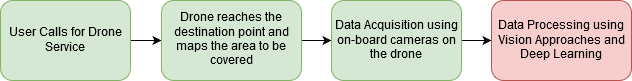
\includegraphics[width=\linewidth]{SummerInterReport/project/Images-Major/Intro_Flow.png}
    \caption{A concise flow of the proposed idea}
    \label{fig:Concise Flow}
\end{figure}

\section{Overview}

Our work compiles a study and explores various developments of a multispectral processing system based on an UAS (Unmanned Aerial System) to perform analysis on agricultural fronts and enable farmers to use smart precision farming. A quadcopter (drone) is used as the UAS where it covers the area based on a service call from the application. The imagery part is achieved by an embedded system, Raspberry Pi, which does the data acquisition and data processing. A modified one camera setup of the NoIR (No InfraRed Filter CMOS sensor) camera has been used for capturing the aerial imagery for computation. A comparative camera study was also performed. The data processing involved comparison of reflectances of Near IR and Red spectra to calculate the NDVI and thereby assess the plant health.


\section{Calling for Drone Service}
An android application serves as the user end application part of the system. It can be used in either Hindi or English to call for the drone service. The application has an easy to use interface where the farmer's phone gets registered automatically as a user and the farmer can call for the drone at his own position using the phone's GPS location. The application allows the user to fetch previous reports from the Firebase storage database or analyze live status of the field analysis over LAN (Local Area Network) connection to the drone in close proximity. In case the farmer doesn't have a smartphone, the system uses Twilio server on python backend for the drone dispatch stations using which, a farmer can send a SMS in a specified format, in which case the service would offer a personnel for operating the drone and presenting the reports to the farmer.
\section{Drone Mapping the area} The drone covers the area autonomously by stably following the geo-location tags based based on GPS computed for its path by the mission planner. We used the ArduPilot APM 2.8 flight controller which has an embedded firmware for stabilizing the drone using various flight modes after callibrating it, analyzing its flight metrics, GPS integration and support for external compass, I2C and telemetry as well. The APM was programmed using open-source software, the firmware ArduCopter 5.3.3 uploaded through Mission Planner based on ArduPilot platform, to first follow the GPS tag to the Field location from the nearest Base Station and then covering the complete area through covering the polygon drawn over the field to be covered or Area Of Interest (AOI) by the path computed.

\section{Data Acquisition} The data acquisition system consists of a Raspberry Pi, A NoIR Pi camera and the trigger from the APM. An open source plugin in Mission Planner, OperDroneMap(ODM) was used to merge the multi-spectral imagery into an orthomosaic from the captured images. 

\section{Data Processing} The data is processed as live time feed of the drone imagery where every frame is computed to yield the infographic feed and the post processing involves combining the individual frames into an orthomosaic covering the entire field using an open source software Fiji or using mathematical modelling of the distance. A developed Python script calculates the Normalized Difference Vegetation Index (NDVI) through the Near InfraRed (NIR) and Red field reflectance spectra collected from the NoIR Pi camera, acting as a metric to define the plant health through chlorophyll level analysis. This NDVI calculation is done both on the frame wise feed and the final orthomosaic. The complete information graphic developed lets the farmer know which areas of the field are poor in chlorophyll and thereby health. Also, we present a water index of the field using only the Near IR spectrum, which is a clear indicator of water's thermal coefficient and thereby the water retention in every region of the crop field. 


%stats1 citation - "India economic survey 2018: Farmers gain as agriculture mechanisation speeds up, but more R&D needed". The Financial Express. 29 January 2018.  https://www.financialexpress.com/budget/india-economic-survey-2018-for-farmers-agriculture-gdp-msp/1034266/

%stats2 citation- "India outranks US, China with world's highest net cropland area". Retrieved 17 November 2018. http://www.indiawaterreview.in/Story/Features/india-outranks-us-china-with-worlds-highest-net-cropland-area/2096/2#.W_A_iOgzZPY

%eighth- Multi Temporal Data wala
\chapter{Related Work}
Remote sensing \cite{two} with the unmanned aerial systems (UAS) with multispectral imagery dates back to 2008 \cite{eight-icuas} and earlier where results were generated using traditional approaches of using high cost wide band multi-spectral cameras with application of physical filtering. The field is now emerging as an application which systematically applies monitoring of vegetation and crops to enable smart decisions for the farmers in the agricultural activities. The field has a  lot of dependence on the satellite imagery for collection of hyperspectral imagery. However, recently the paradigm has shifted to cheaper UAS based solution which is able to gather large amounts of raw data to process for an be used to monitor crop health in more than one way such as water level concentration identification \cite{two-remotev2}, vigor analysis \cite{three-remotev2}, biomass estimation and disease monitoring using algorithmic analysis based on data from hyperspectral and thermal imagery as well as using machine learning applications of clustering (unsupervised) and supervised by collection of large amounts of labelled data of particular fields.  
\\
\\
Both multispectral analysis and the hyperspectral analysis requires acquisition of data aerially, at a fixed position in altitude and coverage of the entire crop field, using low cost passive imagery sensors such as the normal visible light camera (RGB camera), Near Infra Red (NoIR camera) and relatively expensive hyperspectral cameras. The sensors are distinguished by the bands (channels) of electromagnetic spectra reflected by the crop and their corresponding widths. The spatial distribution of the energy reflected by the plants to these sensors differ in the bands of frequency which points to the variation of plant health spatially in the crop field. Each spectrum of energy reaching the sensors are captured based on the specification of the cameras. The multispectral imagery ranges from wide bands 5 to 12 represented as pixels. The hyperspectral imagery has hundreds or even thousands of bands present as narrow width bands (5-20 nm each). The multispectral imagery we use is an adjusted version of the expensive multispectral imagery which only captures the most significant band for chlorophyll reflectance, i.e., the Near IR band. The solution can be used by removing the IR filter present in RGB cameras for the camera to capture the Near IR energy spectrum reflected by the crops as well. This can be isolated from the RGB bands by using a band filter for one of the three visible bands. We used a Red light filter for the same.
\begin{figure}[H]
    \centering
    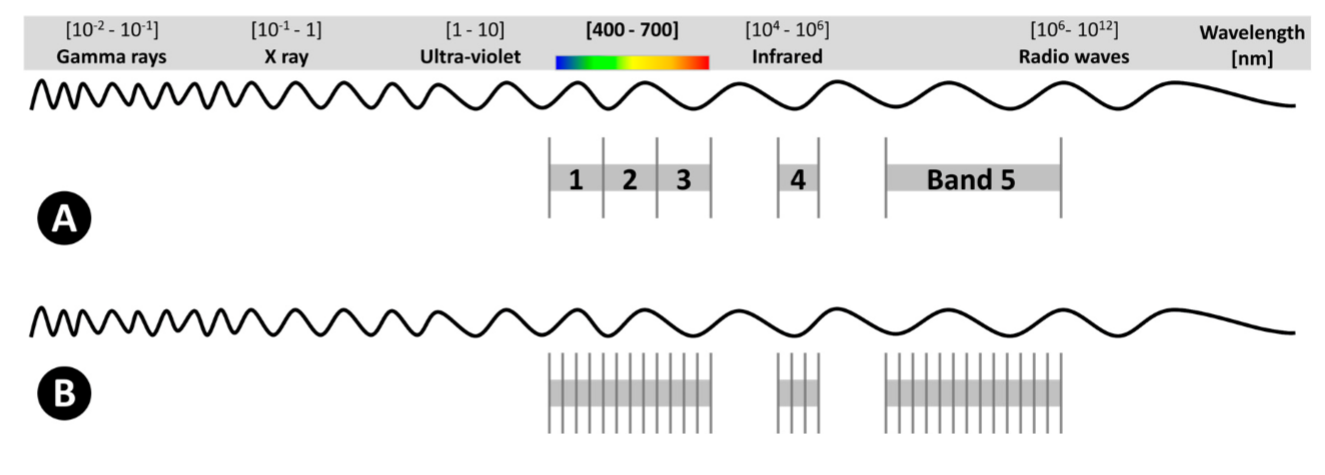
\includegraphics[width=0.7\linewidth]{SummerInterReport/project/Images-Major/em_spectra.png}
    \caption{Spectrum representation including: (A) Multispectral example, with 5 wide bands; and (B) Hyperspectral example consisting of several narrow bands that \cite{fourteen-remotev2}).}
    \label{fig:Concise Flow}
\end{figure}

\\
\\

Both Multispectral and Hyperspectral imagery can be a boon to the agricultural sector over its analysis range to asses even the smallest details such as telling the elemental defciency in the spatial context of the crop to enable precision farming for the individuals. Also, productivity and stress indicators in both agricultural systems can be assessed through photosynthetic light use efficiency quantification, which can be obtained by measuring the Photochemical Reflectance Index (PRI) relying on narrow band absorbance of xanthophyll pigments at 531 and 570nm \cite{fifteen-remotev2}.  However commercial hyperspectral cameras without the acquisition systems and the data processing systems cost upwards of 6000\$, deeming it infeasible in Indian conditions where the infographic of a higher detail would cost leaps more to the farmer as well as would be non-usable due to the higher levels of complexity in data, incomprehensible by a large majority (62\% uneducate as cited by \href{https://timesofindia.indiatimes.com/india/62-farmers-cannot-meet-educational-needs-Survey/articleshow/12049496.cms}{2012 reports of Times Of India}). Commercial multispectral systems costs up to 5000\$ or Rs 3.5 lac however we successfully managed to reduce the expenditure in our system for data acquisition as well as processing to Rs 3000 or 50\$ (using a raspberry Pi 3B+, supporting expansion in ML domains as well fr clustering the hyperspectral imagery in future) and a NoIR camera.
\\
\\
Furthermore, we have used the APM 2.8 flight controllers and tested the algorithms of path planning with Primus V3R in constrained environments as well as CC3D mini, which are cheaper than the commonly used PixHawk or Pixhack flight controllers.





\chapter{System Architecture}

\section{Drone}
%ye daalde Dicky. Himanshu tu bhi padhlio ye summary kal bolne ke lie
%ok
Drones are the quadcopter versions of Unmanned Aerial Vehicles (UAVs) which are used extensively in various fields due to their high maneuverability and stability in almost every conditions. This results their use in a very wide field of applications which asks for high flight times, high altitudes, stable operation and communication. We have explored the drone platform with 3 different flight controllers all of which have been explained in the coming sections. We have also developed a code to fly drones in constrained environment from scratch through python based communication over WiFi for the PID controls, processing on base station (Laptop) and the waypoint navigation with obstacles through Lua Scripting on Open Licensed version of Virtual Robotic Simulator V-REP simulator and emulator through an overhead camera to understand the dynamics of drones in aerodynamical range as well as exploiting the RF communications. We have further used CC3D mini flight controller to fly the drone using in built codes, calibrating the ESCs and the flight controller with the motors on the custom chassis drone we developed the architecture of. We have further moved to the APM 2.8 flight controller to incorporate the GPS control and telemetry extensions. We used Mission Planner to plan the path using a polygon method where the planner automatically divides the whole region and covers the entire area. The Open Drone Map Plugin in Mission planner triggers the data acquisition circuitry to click images and later stitch the orthomosaic. 

\subsection{Waypoint Navigation in constrained environment}
We experimented on the Pluto X drone developed by Dronaviation to undersand the dynamics of drone, code it from scratch to implement the PID algorithm (Propotional-Integral-Derivative Controller algorithm). 
\begin{figure}[H]
    \centering
    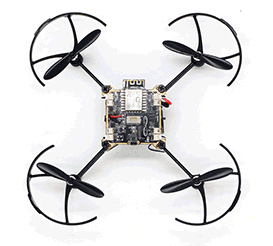
\includegraphics[]{SummerInterReport/project/Images-Major/plutox.png}
    \caption{PlutoX drone from dronaaviation}
    \label{fig:plutox}
\end{figure}
The plutoX drone has the Primus V3R flight controller. It has 16 GPIOs, 2 DAC Channels, 10 DOF Sensor Sui, 4 Mosfet Drivers, 2 UARTS, 20 Pin Header, 4 H Bridge Drivers to connect the Brushless DC motors and 11 Timer Channels. The drone practically presents a 10 minutes flight time with a 800 mAh Lithium Polymer 27C (Lipo battery) with a charge time of 45 minutes. The board has an on-board WiFi module which allows it to communicate over a distance of 60m with any wifi module. 
\\
\\
We use the whole setup in a constrained environment where we are limited by the vision of an overhead camera. For the task of simple waypoint navigation, we present a Whycon coordinate as found out using the Whycon detection script in Robotics Operating System. The position is detected by the python script. The drone is connected to the Laptop through Wifi connectivity and has a Whycon marker above it.
\begin{figure}[H]
    \centering
    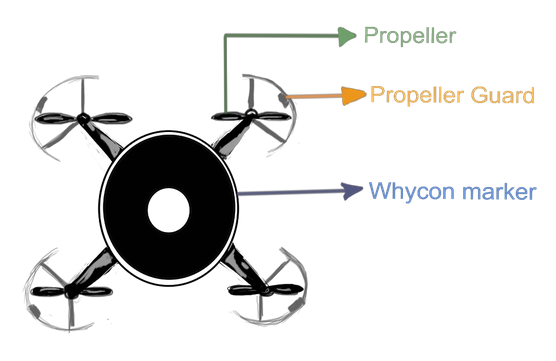
\includegraphics[scale=0.6]{SummerInterReport/project/Images-Major/whycon_plutox.png}
    \caption{PlutoX drone with Whycon Marker schematic}
    \label{fig:plutox_whycon}
\end{figure}
We calculate the error of the drone's current position, as given by the current detected whycon coordinates from the overhead camera, as compared to the waypoint it has to reach. This error is fed to the PID controller in derivative, current and iterative sum form. The PID controller algorithm we developed finds the throttle, pitch and yaw values to be given to the drone to make it traverse to the given waypoint. The given four channel values are given to the drone by the laptop as RC commands from the RC WiFi communication built by the drone.
\\
\begin{figure}[H]
    \centering
    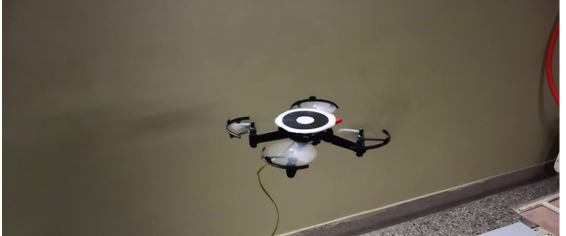
\includegraphics[]{SummerInterReport/project/Images-Major/Flying_pluto.png}
    \caption{PlutoX drone mid-flight}
    \label{fig:plutox_flying}
\end{figure}


The complete experimental setup is made such that the drone employs a whycon marker over it for the camera to identify. The environment is populated with hoops through which the drone has to pass with given positions and orientations. The positions of the hoops are set-up initially via the whycon markers and the orientations are st-up ia the Aruco markers. The python code identifies the positions and orientations and sends the same over ROS to the Coppepelia Robotics' Virtual Robotics simulator, V-REP (Virtual Robotics Emulation Platform). The Lua Script we developed takes in the positions and the orientations and convert them to V-REP's frame of reference using mathematical models. The Overhead camera also has a fish-eye effect which is corrected. The coordinates present are in the following form:
\begin{figure}[H]
    \centering
    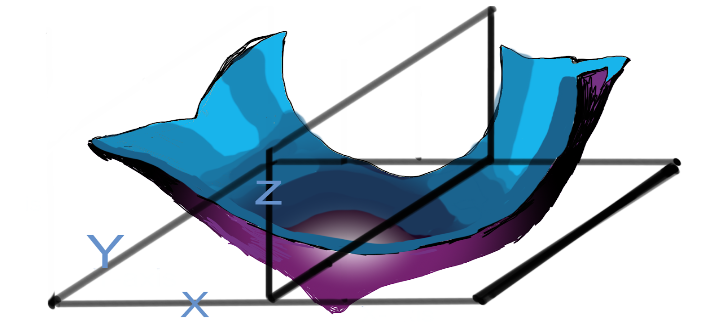
\includegraphics[scale=0.6]{SummerInterReport/project/Images-Major/varz.png}
    \caption{Variation in Z-axis with respect to x-y plane}
    \label{fig:varz}
\end{figure}
\begin{table}[H]
    \centering
    \begin{tabular}{|c|c|}
     \hline
     \textbf{Position} & \textbf{Whycon Z Coordinate}  \\
     \hline
     Centre & 33.47\\
     Top-left & 29.80\\
     Top-right & 30.82\\
     Bottom-left & 29.42\\
     Bottom-right & 29.58\\
     \hline
    \end{tabular}
    \caption{Variation of Z axis with x-y plane}
    \label{tab:varz}
\end{table}

The lua script then places the hoops and the obstacles (in similar way) in the virtual scenario. It then devises the path to the loops in the fashion we give the command to through designating several waypoints in the path. The waypoints are programmable and are devised such that there is no collision with the obstacles by making collision pairs in the 6D state space defined in the Virtual scene itself. The waypoints in the paths are communicated back to the python script which again follows the PID algorithm to cover the waypoints one by one by reducing the errors. The setting up of each stage is explained through flowcharts in the following. Hoops are called trees here.

\begin{figure}[H]
    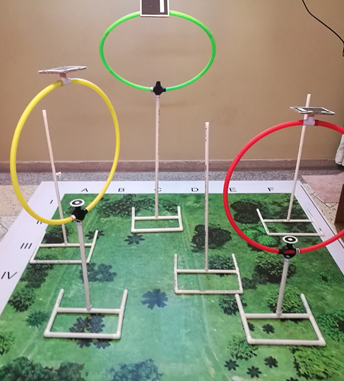
\includegraphics[scale=0.9]{SummerInterReport/project/Images-Major/arena.png}
    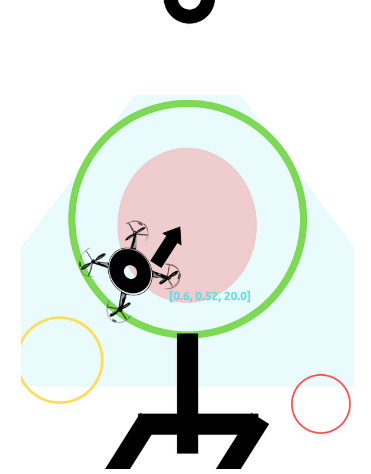
\includegraphics[scale=0.9]{SummerInterReport/project/Images-Major/eyflow.png}
    
    \caption{L: Arena Image with hoops and obstacles; R: Overhead camera and hoop navigation}
    \label{fig:arena}
\end{figure}

\begin{figure}[H]
    \centering
    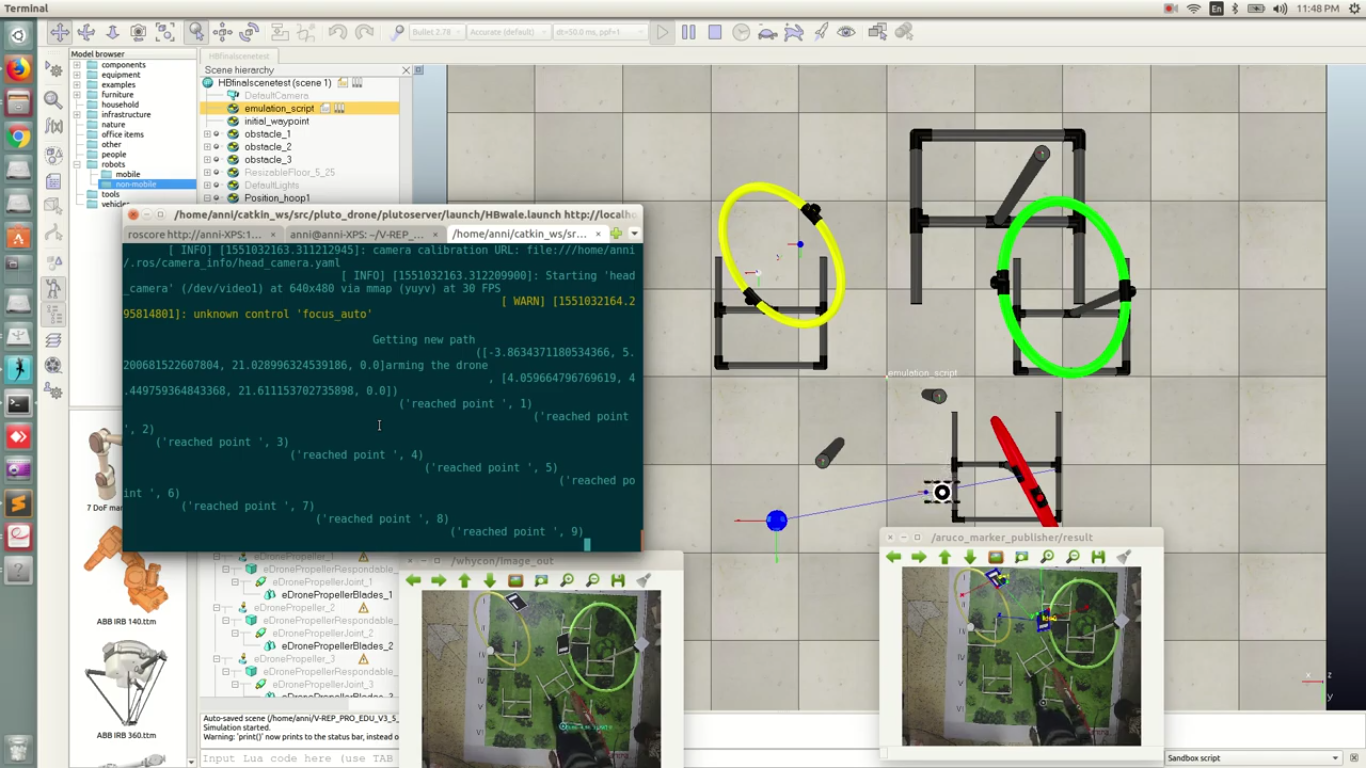
\includegraphics[width=\linewidth]{SummerInterReport/project/Images-Major/simul.png}
    \caption{Simulation and Emulation in V-REP}
    \label{fig:simul}
\end{figure}
\begin{figure}[H]
    \centering
    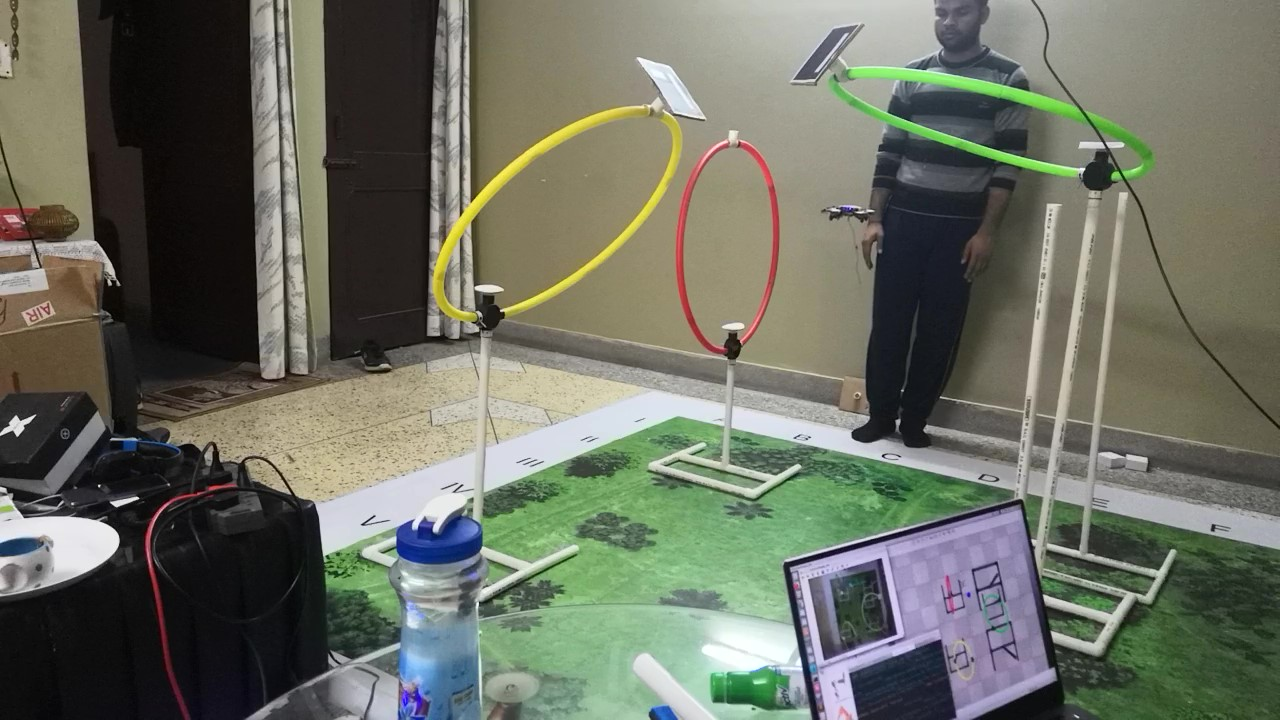
\includegraphics[width=\linewidth]{SummerInterReport/project/Images-Major/finalarena.jpeg}
    \caption{Traversal of PlutoX through designed arena}
    \label{fig:simul}
\end{figure}
\begin{figure}[H]
    \centering
    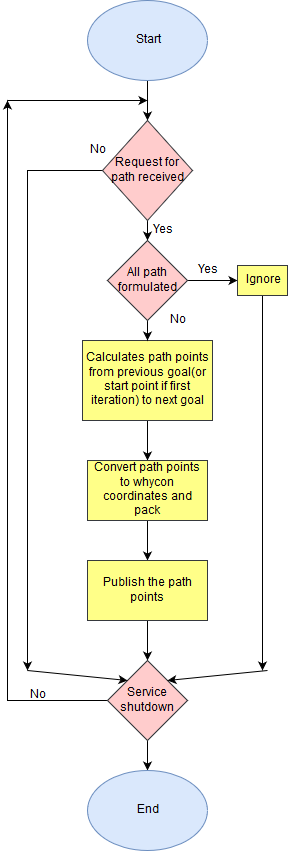
\includegraphics[]{SummerInterReport/project/Images-Major/pathplan.png}
    \caption{Path planning in Lua Script}
    \label{fig:pathPlan}
\end{figure}

\begin{figure}[H]
    \centering
    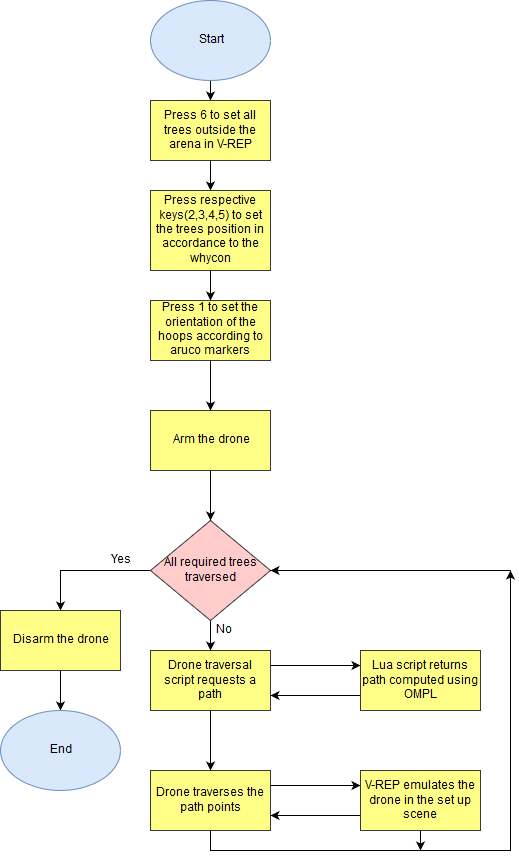
\includegraphics[]{SummerInterReport/project/Images-Major/completeEy.png}
    \caption{Complete experimental flow of constrained waypoint navigation}
    \label{fig:compEy}
\end{figure}

\subsection{PID Tuning - Mathematics}
Systems can broadly be divided into two types; \textbf{open loop systems} and \textbf{closed loop systems}. An open loop system, also called an uncontrolled system, is one in which there is no feedback from the output of the system to the input. A closed loop system on the other hand is a controlled system which has receives a feedback of its operation at every point of time. PID (Proportional-integral-derivative) Controllers are a type of close loop systems. They are used widely in automation industries, aviation industries and other technologies where a feedback is required due to their robust nature covering a diverse range of operations and the ease with which they are implemented. They can be used in any application which requires a feedback mechanism to take control of the rise times, over-shootings, steady-state errors and oscillations damping.
\\
\textbf{Types of Controllers}
\begin{itemize}
    \item \textbf{Proportional Controller (P Controller)} \\
    P controller is mostly used in first order processes with single energy storage to stabilize the unstable process. The main usage of the P controller is to decrease the steady state error of the system. As the proportional gain factor K increases, the steady state error of the system decreases. However, despite the reduction, P control can never manage to eliminate the steady state error of the system. As we increase the proportional gain, it provides smaller amplitude and phase margin, faster dynamics satisfying wider frequency band and larger sensitivity to the noise. We can use this controller only when our system is tolerable to a constant steady state error. In addition, it can be easily concluded that applying P controller decreases the rise time and after a certain value of reduction on the steady state error, increasing K only leads to overshoot of the system response. P control also causes oscillation if sufficiently aggressive in the presence of lags and/or dead time. The more lags (higher order), the more problem it leads. Plus, it directly amplifies process noise. 
    \item \textbf{Proportional Derivative Controller (PD Controller)} \\
    The aim of using P-D controller is to increase the stability of the system by improving control since it has an ability to predict the future error of the system response. In order to avoid effects of the sudden change in the value of the error signal, the derivative is taken from the output response of the system variable instead of the error signal. Therefore, D mode is designed to be proportional to the change of the output variable to prevent the sudden changes occurring in the control output resulting from sudden changes in the error signal. In addition D directly amplifies process noise therefore D-only control is not used.
    \item \textbf{Proportional Integral Derivative (PID Controller)}\\ P-I-D controller has the optimum control dynamics including zero steady state error, fast response (short rise time), no oscillations and higher stability. The necessity of using a derivative gain component in addition to the PI controller is to eliminate the overshoot and the oscillations occurring in the output response of the system.
\end{itemize} 
\\
\textbf{Equations and Diagrams}
\begin{enumerate}
    \item \textbf{P controller}\\
    A P controller consists of only a linear gain Kp. The output of such controller can be simply given as\\
    \begin{equation}
        output = Kp * error
    \end{equation}
    \begin{figure}[H]
        \centering
        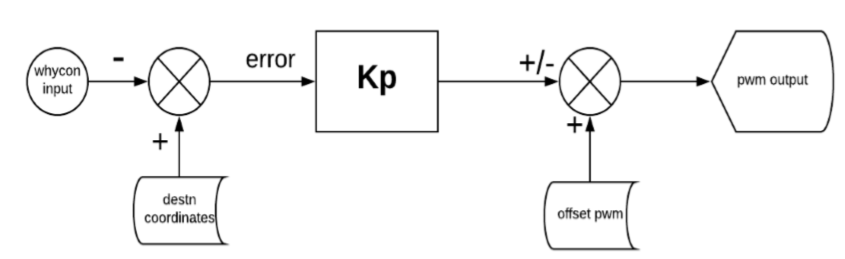
\includegraphics[width=0.8\linewidth]{SummerInterReport/project/Images-Major/pblock.png}
        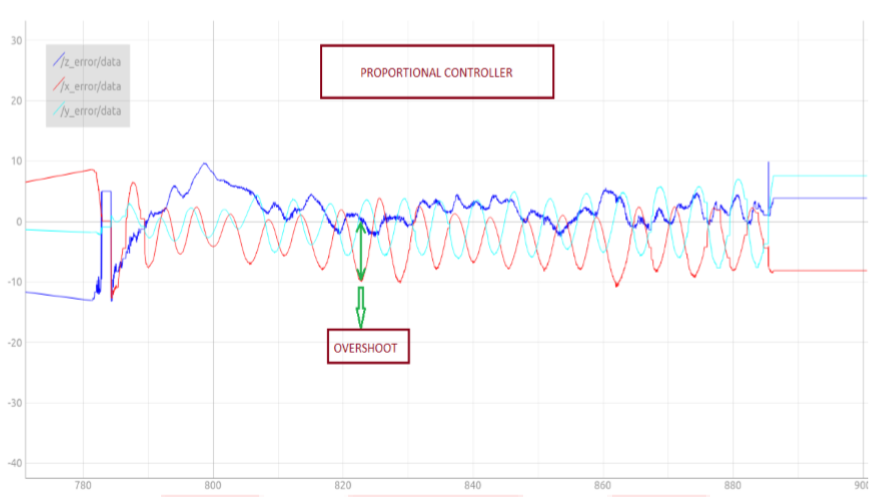
\includegraphics[width=0.8\linewidth]{SummerInterReport/project/Images-Major/pgraph.png}
        \caption{P controller Block Diagram and Graph}
        \label{fig:Pcontroller}
    \end{figure}
    The whycon input consists of x, y and z coordinates which gives the current location of the drone. Suppose the destination is say, (x1, y1, z1), then the difference of coordinates i.e (x1-x) ,(y1-y), (z1-z) will be fed as an input to the P-controller. The resultant product i.e Kp * error will be added or subtracted to the offset pwm as the need be to give the final output.
    
    \item \textbf{PD Controller}\\
    Oscillations can be damped by using a differential gain along with the P-Controller. The system as a whole is said to be a PD Controller.
    \begin{figure}[H]
        \centering
        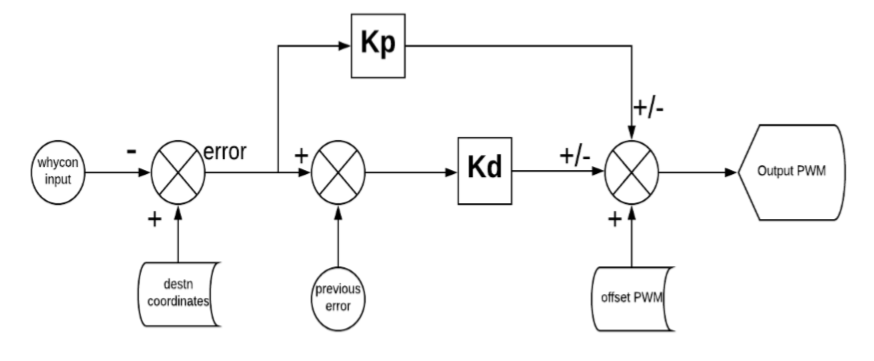
\includegraphics[width=0.8\linewidth]{SummerInterReport/project/Images-Major/dblock.png}
        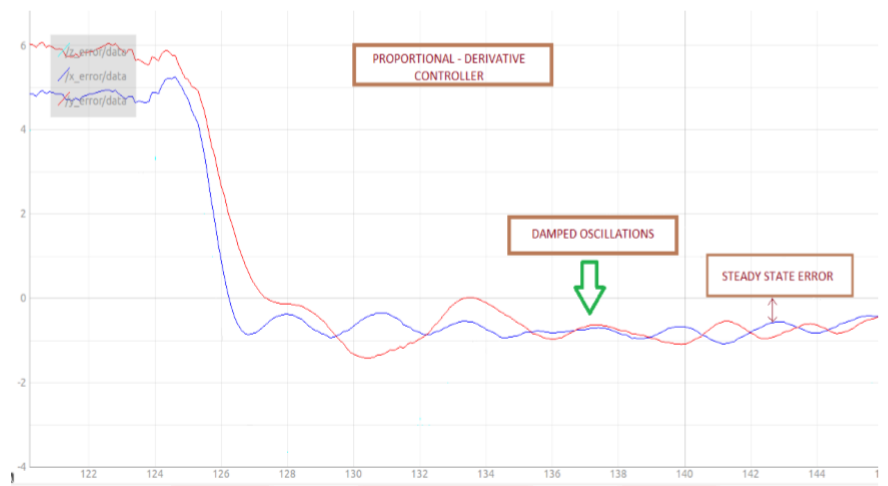
\includegraphics[width=0.8\linewidth]{SummerInterReport/project/Images-Major/dgraph.png}
        \caption{PD controller Block Diagram and Graph}
        \label{fig:PDcontroller}
    \end{figure}
    The differential gain Kd is multiplied with the difference of error and previous error. Previous error is a variable that holds the last error generated by the controller output.\\
    The controller output in this case is given as
    \begin{equation}
        output = Kp * error + Kd * (error - previous error)
    \end{equation}
    Note that Kd is calculated keeping the sampling time in consideration. This output will be further added or subtracted to the offset pwm as the need be to give the final output.
    
    \item \textbf{PID Controller}\\
        In order to minimise the steady state error we introduce another gain called Ki ,the integral gain. Such a system is said to be a PID Controller
        \begin{figure}[H]
        \centering
        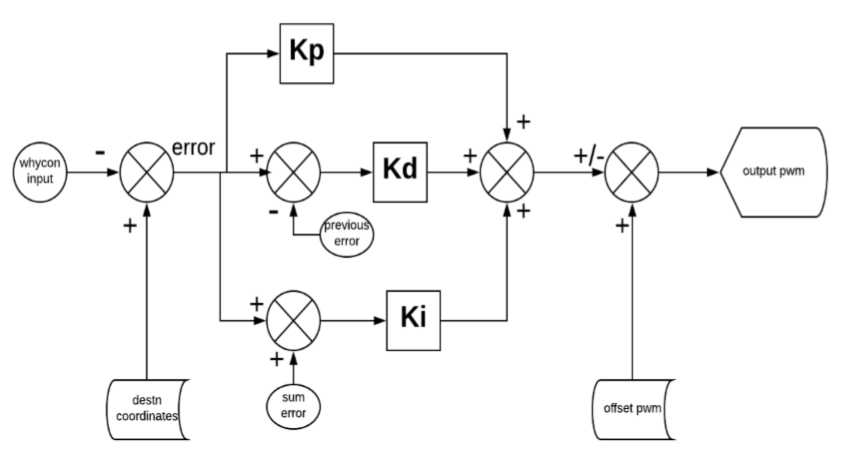
\includegraphics[width=0.8\linewidth]{SummerInterReport/project/Images-Major/pidblock.png}
        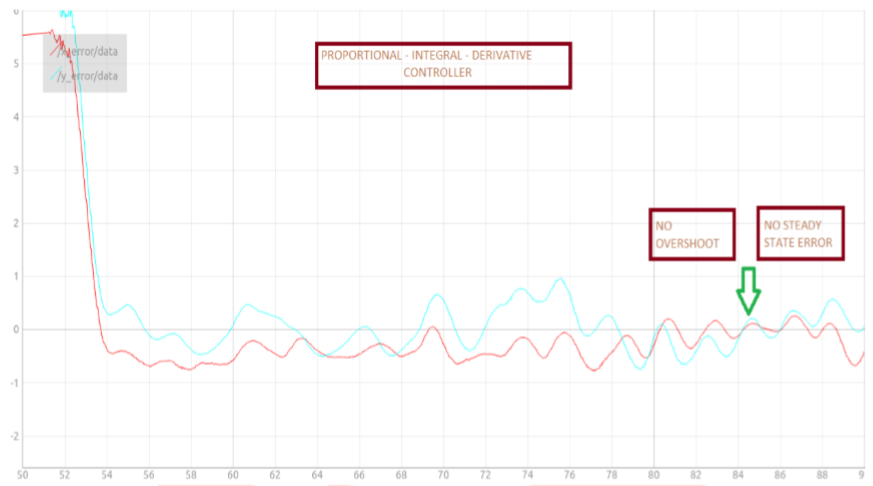
\includegraphics[width=0.8\linewidth]{SummerInterReport/project/Images-Major/pidgraph.png}
        \caption{PID controller Block Diagram and Graph}
        \label{fig:PIDcontroller}
    \end{figure}
    Here in we keep track of the error over time i.e. sum up the errors over a specified sampling time.
    \begin{equation}
        Iterm = (Iterm + error) * Ki
    \end{equation}
    Note that Ki is calculated keeping the sampling time in consideration. This output will be further added or subtracted to the offset pwm as the need be to give the final output.
    \begin{equation}
        output = Kp*error + Iterm + Kd*(error - previous error)        
    \end{equation}


\end{enumerate}


















\subsection{Drone architecture and components}
In order to successfully navigate through the field, we need to ensure a drone with all the parts intact which are distinctive for each size of the drone. We have used the 250mm or the 25cm Carbon Fiber Chassis of the drone to build a sturdy, powerful and small drone, capable of doing everything with lesser power utilization, greater flight times and better handling at constrained areas. We use the quad-copter in X-copter fashion, meaning that two peds of the quad-copter would face the front hen we give it a pitch and a X orientation is followed at all times, no individual leg leans on giving it pitch, roll or yaw. 
\begin{figure}[H]
    \centering
    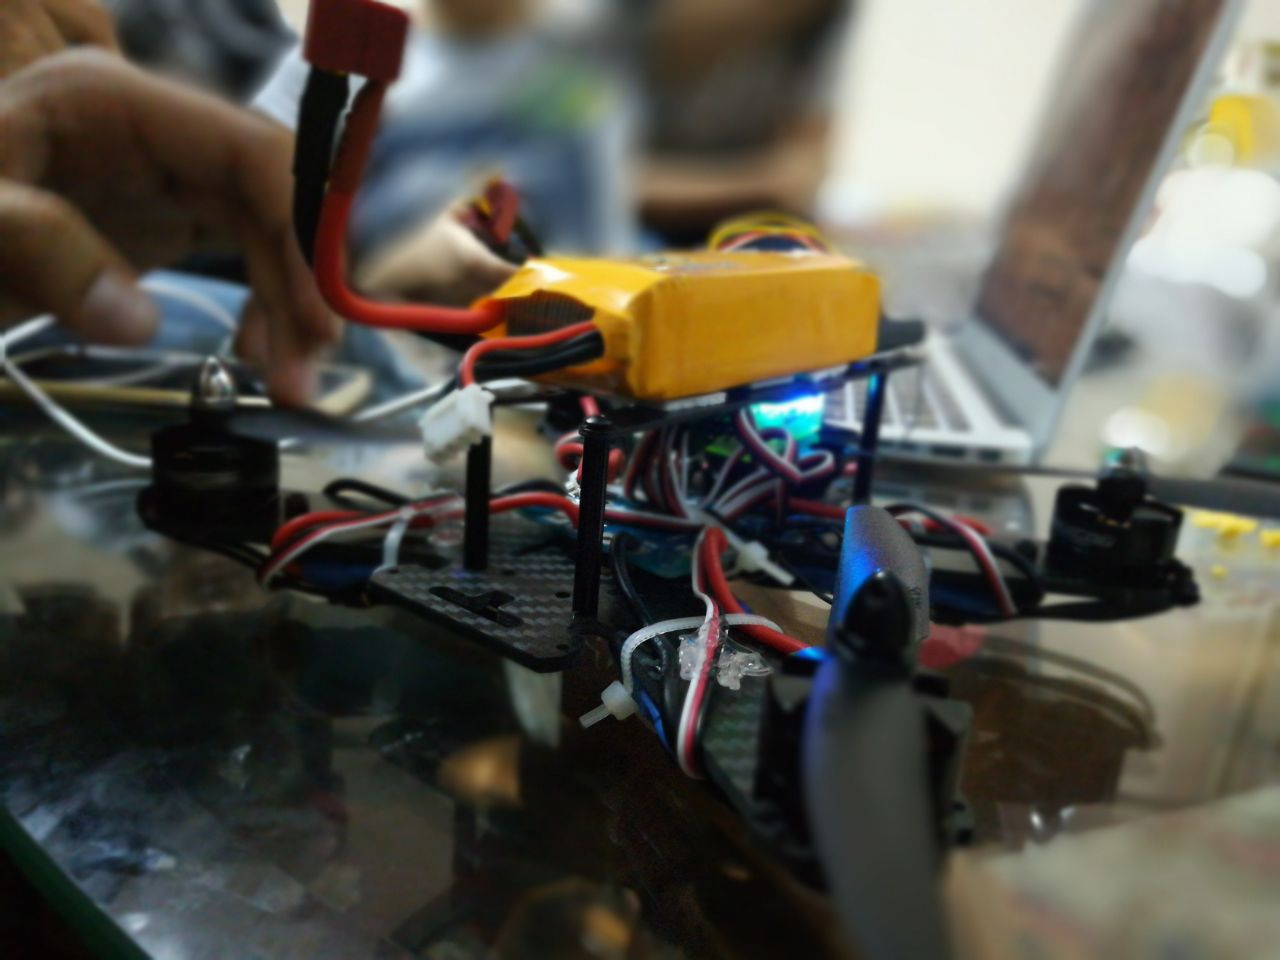
\includegraphics[width=0.8\linewidth]{SummerInterReport/project/Images-Major/drone.jpeg}
    \caption{Custom 250mm drone}
    \label{fig:drone}
\end{figure}
The components used are-
\\
\begin{enumerate}
    \item \textbf{Standard Prop}\\
    The propellers are specifically designed wings of the drone. The propeller design is based on the direction of the circular motion, either it is clockwise or anti-clockwise. The propellers are made from high grade plastics to avoid breaking on crashes. They have an aerodynamic body due to a lean in their horizontal axis to either inwards or outwards based on which, they are fixed on Clockwise or Counter Clockwise motors. The lean is such that the propellers always push air in a downward direction when fixated on the designated clockwise or the anticlockwise motor. This provides necessary thrust for the drone to take off, increase altitude or change its direction. We have used both Two Blade and Three-bladed propellers of 2.2cm single wing span.
    \item \textbf{Brushless DC Motors (BLDC Motors)}\\
    We used high power (2200 kV) brush less DC motors in order to levitate the drone along with the body and attachment payload. To make a drone fly, the rotation of all the motors should oppose the oppose the rotation to the adjacent motors. The given motors were connected specifically to the clockwise and counter-clockwise directions.
    \begin{figure}[H]
    \centering
    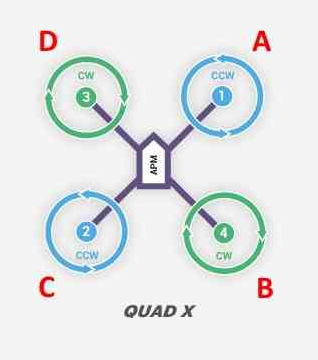
\includegraphics[]{SummerInterReport/project/Images-Major/motors.png}
    \caption{Drone BLDC motor connections}
    \label{fig:motors}
\end{figure}
    \item \textbf{Electronics Speed Controllers(ESC)}\\
    An electronic speed controller or ESC is an electronic circuit with the purpose to vary an electric motor's speed, its direction and possibly also to act as a dynamic brake. It converts DC battery power into 3-phase AC for driving brushless motors. It offer high power, high frequency, high resolution 3-phase AC power to the motors in an extremely compact miniature package. We used Rapid ESCs with high current ratings (3A) to drive the motors. They basically acts as the motor driver circuits in drone with PWM signalling in rapid fashion. The ESC gets power from the LiPo battery and have a signalling wire as well.
    \item \textbf{Battery}\\ 
    We used Lithium polymer (LiPo) batteries, It offer the best combination of energy density, power density. It also gives the optimal flight time to cover the planned area. The LiPo battery we used had a 2200 mAh capacity with a 20C rating.
    \item \textbf{Power Distribution Board}\\
    It acts as the intermediatory between the LiPo battery, the ESCs and the other electronic circuitry like GPS, receivers and the flight controller on board the drone.
    \item \textbf{Transmitter-Receiver or GPS}\\
    These are used to give direction to the drone. We initially used a FlySky transmitter-Receiver at 2.4 GHz for manually giving the 6 channel input (including throttle, pitch, roll and yaw) commands to the drone. For automated controls, a GPS was used along with Mission Planner software to plan the path and burn this updated firmware into the flight controller for it to follow the path. 
    \item \textbf{Flight Controller} \\
    We tried using CC3D Mini as well as APM2.8, both of which are discussed in the further sections.
\end{enumerate}

\begin{figure}[H]
    \centering
    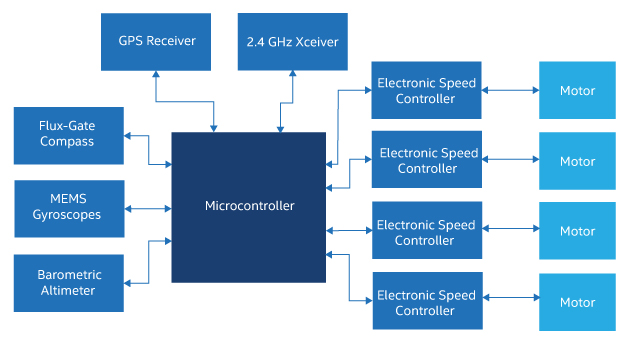
\includegraphics[]{SummerInterReport/project/Images-Major/block.png}
    \caption{Architecture Overview from System Design Journal - Intel
us-systemdesign-journal-drones-f1}
    \label{fig:compEy}
\end{figure}


\subsection{CC3D mini Flight Controller}
The CopterControl, CC3D and mini CC3D flight controllers are all types of stabilisation hardware which run the OpenPilot firmware. They can be configured to fly any airframe from fixed wing to an octocopter using the OpenPilot Ground Control Station (GCS) software. The CopterControl was the first generation board, which ceased manufacture in 2012 due to lack of availability of the gyro sensors used for stabilisation. The board design was then revised and released with an improved gyro sensor which is less affected by temperature changes. This revision is called the CC3D, and apart from the gyro sensor change is identical to the original CopterControl.
\\
We used the CC3D Mini board which is as cheap as Rs 700 or 10\$ and contains the firmware to fly the drone manually using a transmitter-receiver. GPS cannot be integrated with this flight controler, hence we depreciated it of its use in our work. 

\begin{figure}[H]
    \centering
    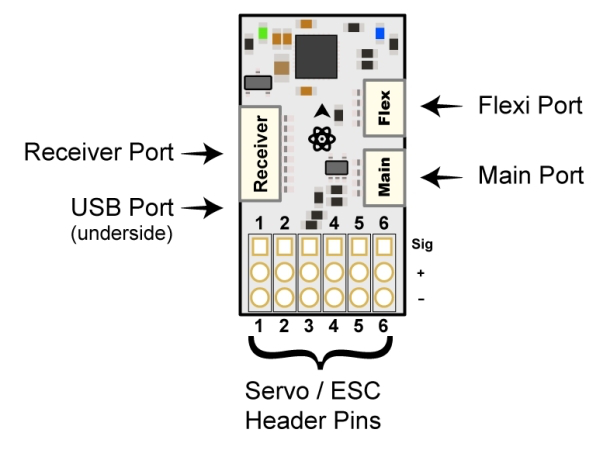
\includegraphics[scale=0.35]{SummerInterReport/project/Images-Major/cc3d.png}
    \caption{Schematic of mini cc3d (Source: DroneTrest)}
    \label{fig:compEy}
\end{figure}
\subsection{APM 2.8 Flight Controller}
Ardupilot Mega (APM) is a professional quality IMU autopilot that is based on the Arduino Mega platform.  This autopilot can control fixed-wing aircraft like drones, multi-rotor helicopters, as well as traditional helicopters.  It is a full autopilot capable for autonomous stabilisation, way-point based navigation and two way telemetry with Xbee wireless modules. It supports 8 RC channels with 4 serial ports. It is our main choice of Flight controller due to it's \textbf{advancements over the CC3D mini.}
\\
It is an open source autopilot firmware that supports planes, multicopters with full mission scripting over point-and-click. It Can support hundreds of 3D waypoints and also Autonomous takeoff, landing and special action commands such as video and camera controls. There is presence of automatic modes like loitering, stabilization, altitude-hold, Return-To-Launch over manual control and accurate GPS waypoint mapping in autonomous conditions.
\\
Ardupilot works on the ArduCopter 5.3.3 firmware which is installed with the help of mission planner. The firmware is the code that runs on the board as a permanent embedded software. Depending on what code we load, we can use the APM to control fixed wing aircraft, multi rotors, helicopters and also ground rovers. We use ArduPilot Mission Planner to update the firmware on the board. The APM board is based on Atmega2560 chip with a small on-board flash memory of 128kB and 16kBs of RAM.
\\ 
The APM 2.8 Board has extension ports for Telemetry, External I2C port, Old and New GPS port, a USB port for uploading the firmware and mission, and other GPIO pins as well to support expandability.

\begin{figure}[H]
    \centering
    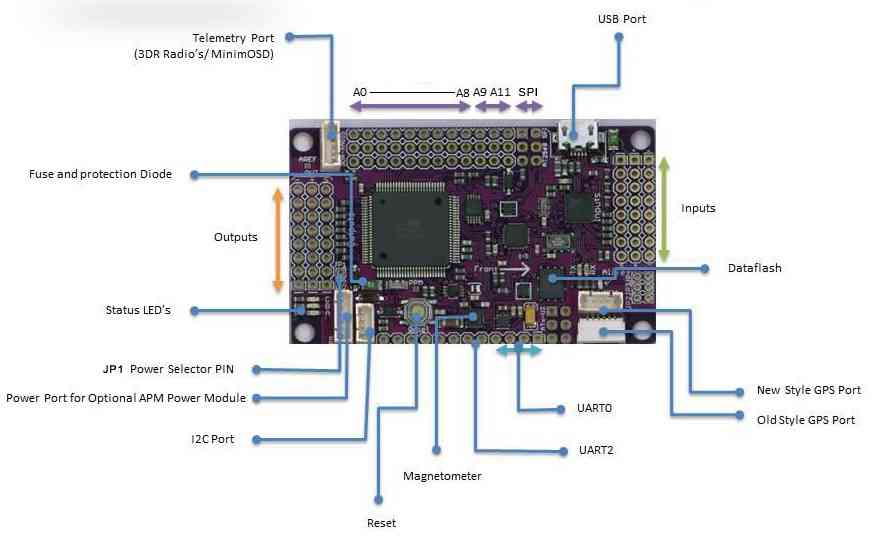
\includegraphics[scale=0.7]{SummerInterReport/project/Images-Major/apm.jpg}
    \caption{Schematic of APM2.8 (Source: ArduPilot)}
    \label{fig:apm}
\end{figure}
\subsection{GPS and Mission Planner}
For navigation of drone and monitoring the field, we use Ublox M8N GPS module. which is highly sensitive and its gives highly accurate position of the navigating drone. The GPS module is high precision and gives low errors to ensure safe flight. It is used for reaching the given point as well as mapping the whole area and covering it.
\\
Mission Planner is a ground control station for Plane, Copter and Rover. It is compatible with Windows only. Mission Planner can be used as a configuration utility or as a dynamic control supplement of the autonomous vehicle. For initial setup-
\begin{enumerate}
    \item Load the firmware (the software) into the APM2.8
    \item Setup, configure, and tune the motors and ESCs of the Drone and the transmitter controls.
    \item Plan, save and load autonomous missions into autopilot with simple point-and-click way-point entry on Google or other maps.
    \item Download and analyze mission logs created by autopilot.
    \item Interface with a PC flight simulator to create a full hardware-in-the-loop UAV simulator.
\end{enumerate}

With appropriate telemetry hardware, we can also Monitor drone status while in operation and record telemetry logs which contain much more information of the on-board autopilot logs. 
\begin{figure}[H]
    \centering
    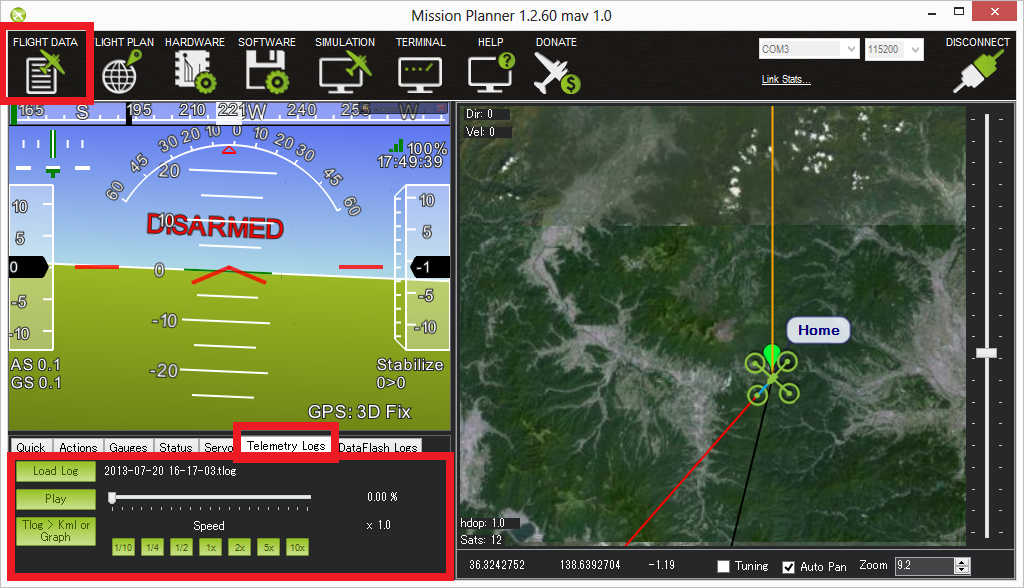
\includegraphics[width=\linewidth]{SummerInterReport/project/Images-Major/mp1.png}
    \caption{Mission Planner GUI(Source: ArduPilot)}
    \label{fig:compEy}
\end{figure}

\begin{figure}[H]
    \centering
    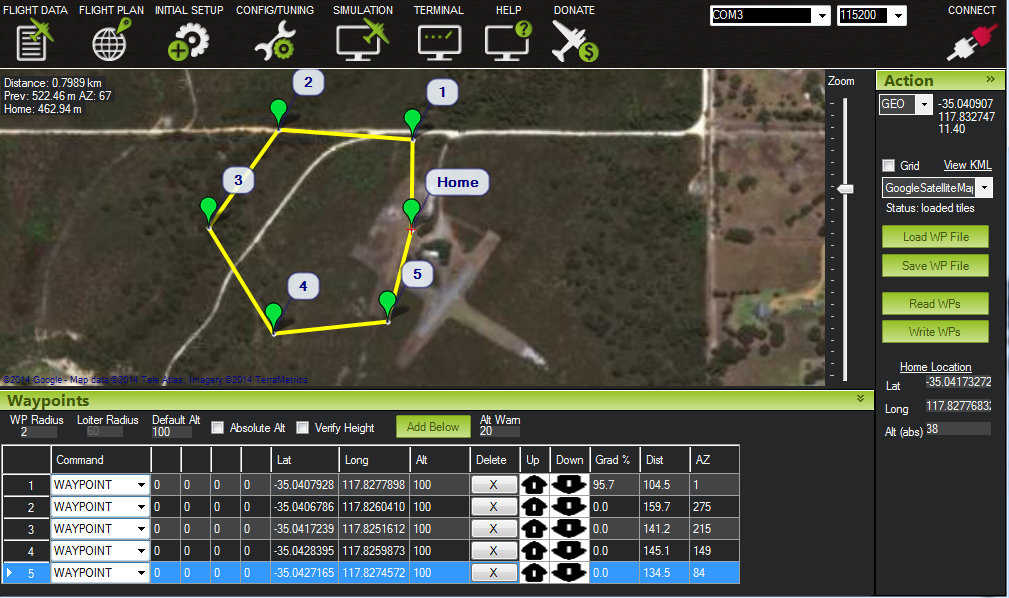
\includegraphics[width=\linewidth]{SummerInterReport/project/Images-Major/mp2.png}
    \caption{Planned Mission (Source: ArduPilot)}
    \label{fig:compEy}
\end{figure}

\section{Data Acquisition and Processing System}
The Data Acquisition and Processing System consists of a Raspberry Pi 3B model, a Picam version 2 RGB camera and a Pi NoIR Camera. These cameras were used due to their low costs (7\$ and 10\$ respectively), low weight and direct connectivity to Pi's GPU using the CSI port for communication, which makes them the fastest and the best alternatives available. These cameras were located at the bottom of the drone setup in an encasing we designed to keep the set-up expandable and safe on landing.
\begin{figure}[H]
    \centering
    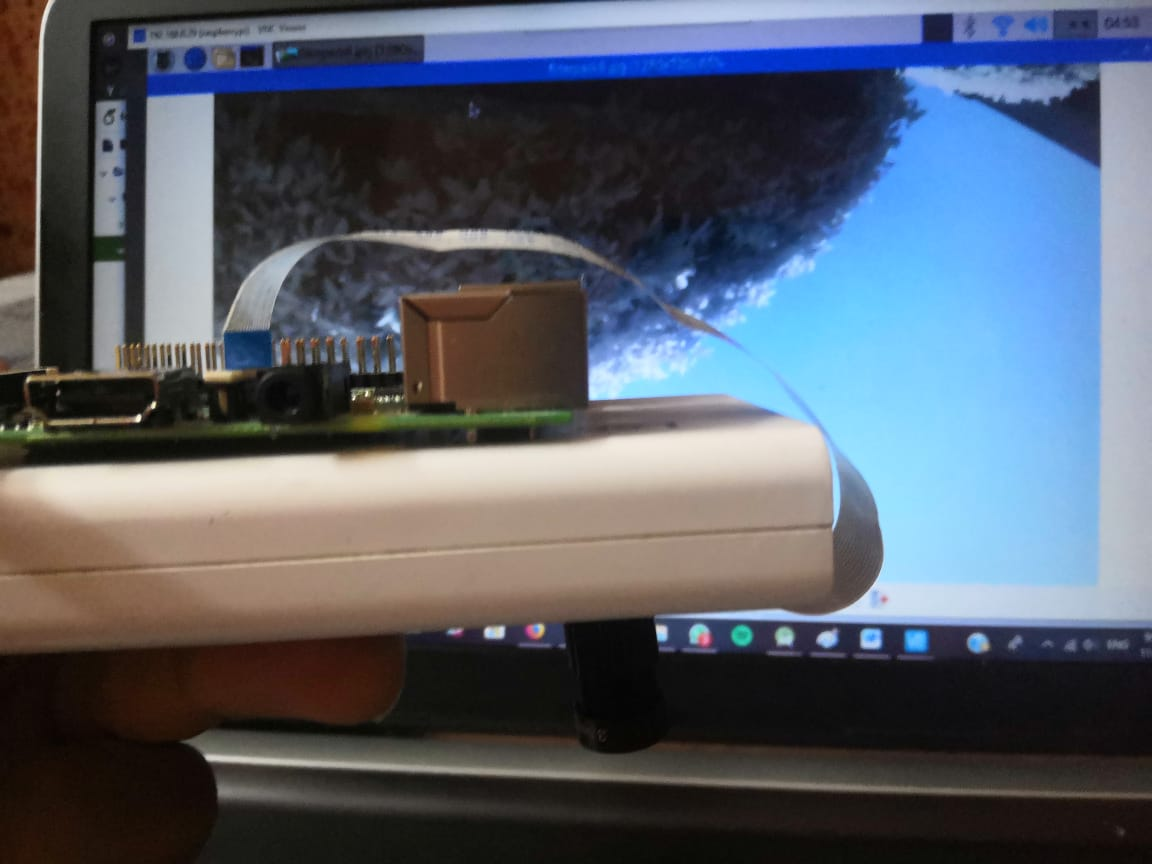
\includegraphics[width=0.7\linewidth]{SummerInterReport/project/Images-Major/pi_system.jpeg}
    \caption{Data Acquisition and Processing System}
    \label{fig:compEy}
\end{figure}

\subsection{Raspberry Pi}
 The Raspberry Pi is used to collect the data and act as the trigger. It detects the trigger event by the flight controller and then capture images with time and GPS stamp. Raspberry Pi 3B is a microcomputer which can run on any OS. We selected the native Raspbian OS to operate the Pi. We used the high speed CSI port (Camera Serial Interface). It is a specification of the Mobile Industry Processor Interface (MIPI) Alliance. It defines an interface between a camera and a host processor. The CSI port in Pi connects the camera directly with the VideoCore IV GPU of the Raspberry Pi.
 \begin{figure}[H]
    \centering
    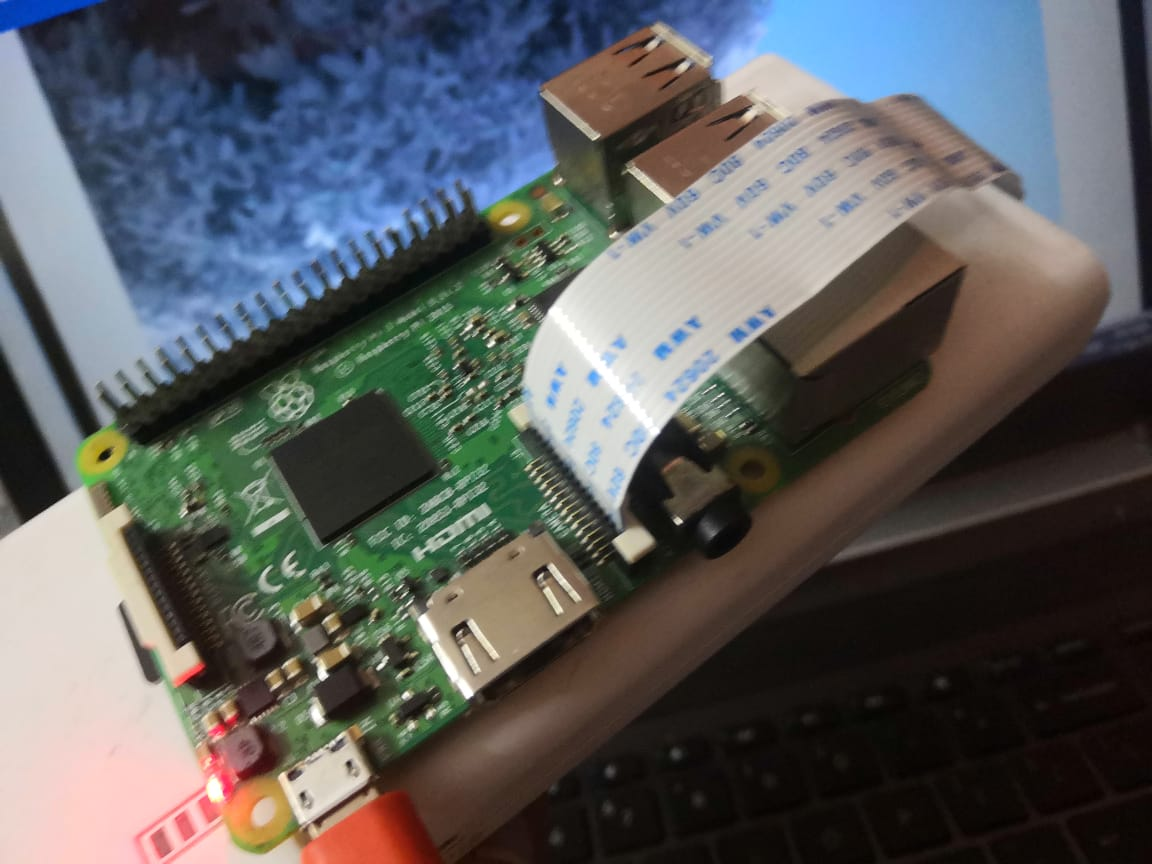
\includegraphics[width=0.5\linewidth]{SummerInterReport/project/Images-Major/pi_top.jpeg}
    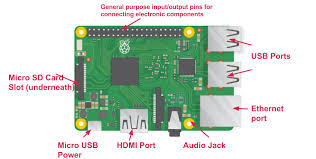
\includegraphics[width=0.5\linewidth]{SummerInterReport/project/Images-Major/pi.jpg}
    \caption{RaspberryPi 3B}
    \label{fig:compEy}
\end{figure}
 The 3B model of Raspberry Pi has the following specifications relevant for data processing and acquisition:
 \begin{itemize}
     \item Quad Core 1.2GHz Broadcom BCM2837 64bit CPU
     \item 1GB RAM
     \item BCM43438 wireless LAN and Bluetooth Low Energy (BLE) on board for communication purposes for live feed analysis.
     \item 40-pin extended GPIO
     \item CSI camera port for connecting a Raspberry Pi camera
     \item Micro SD port for loading your operating system and storing data
     \item 4 USB 2 ports
 \end{itemize}
\subsection{NoIR Camera}
The Pi NoIR gives everything the regular RGB Camera Module offers, with one difference: it does not employ an infrared filter. (NoIR = No Infrared.) This means that pictures we take contains the Near Infra Red component in the taken pictures. We also employ a red light filter to block off all extra incoming light. The sensor used is a 5-megapixel OmniVision OV5647 sensor.
\begin{figure}[H]
    \centering
    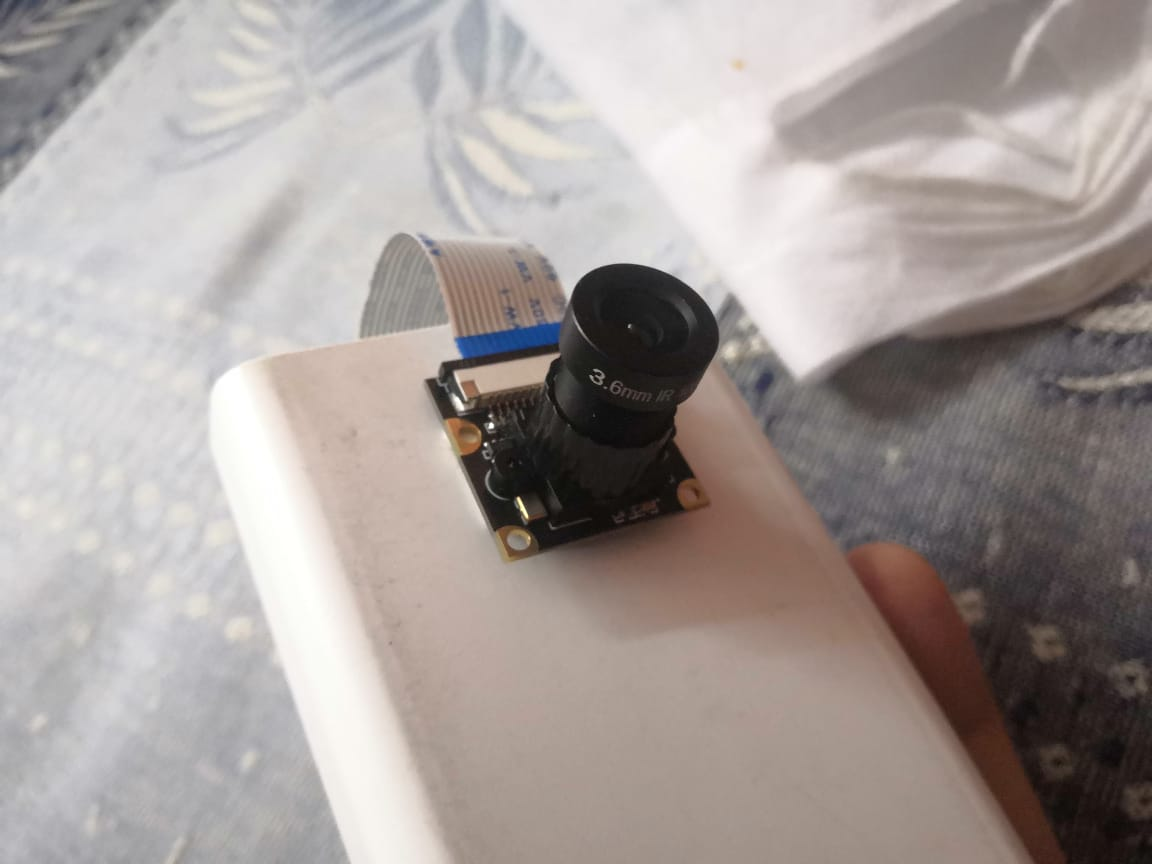
\includegraphics[width=0.7\linewidth]{SummerInterReport/project/Images-Major/pi_bottom.jpeg}
    \caption{NoIR Camera}
    \label{fig:compEy}
\end{figure}
\section{Android Application}
The android application contains the following codes:
\begin{enumerate}
    \item GPS fetching code
    \item Firebase connectivity to fetch older reports
    \item Hindi Text views and Buttons to support Bilungistic approach
    \item Web View over LAN and a given port to show the live feed of the processed NDVI
\end{enumerate}
\chapter{Methodology}
We developed a drone based monitoring and visualization service for the farmers using an easy to use interface of android application. The application serves as an intermediary between the local Drone dispatch station. The dispatch stations are already present in Uttrakhand as UKSWAN (Uttrakhand State Wide Area Network).\\ 
Drone based scanning of a large area using both visible and near-infrared light by stitching images on basis of their location could help track changes in plants at large scale and identify the distribution pattern very precisely.\\
The whole process can be broken down in steps, starting with polygon formation of the area to be processed or the crop cover. Trajectory of the Drone is planned by an open source library Mission Planner with a ground station interface compatible with ArduPilot platform tended to be the basic wireline platform of the drone. Flight trajectories are planned by polygon points in the AUTO mode of the drone flight. The drone is a 250mm chassis drone equipped with an  ArduPilot based flight controller, APM 2.8 which can be given GPS coordinates of the points to be traversed through a remote server (can be a phone) or through direct instructions to the flight controller before beginning the flight using the firmware ArduPilot 5.3.3. We use NoIR camera with a  blue filter, allowing for only near Infra-Red wavelengths to be captured. We use a Raspberry Pi to trigger the cameras to capture the images of the field in their field of vision at particular distances covered by the drone. Hence, as the drone travels the trajectory planned by Motion Planning library to cover the crop field, images are taken by the drone in RGB, near IR. It is to be noted that no images are processed or uploaded to the cloud in between the flight as a high processing or high power circuitry restrict the flight time of the drone, allowing for only small crop fields to be covered, thus making the service infeasible.
The taken images are then collected according to the optimum levels of frontal and side overlaps (60\% and 35\% respectively) for stitching the images into one image.\\
\begin{figure}[H]
    \centering
    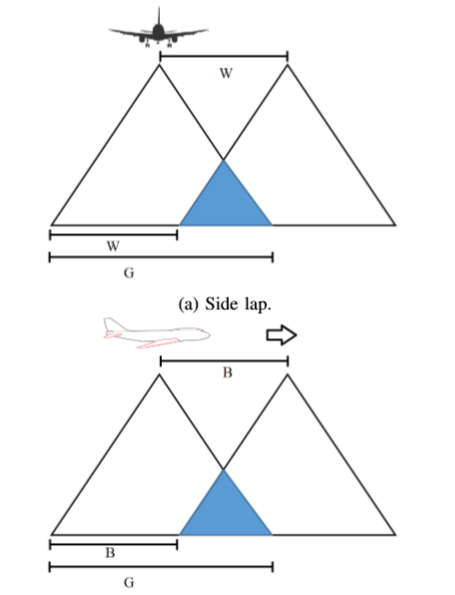
\includegraphics[width=0.7\linewidth]{SummerInterReport/project/Images-Major/overlap.png}
    \caption{Overlap and Stitching Source: \cite{one}}
    \label{fig:compEy}
\end{figure}

For the near IR and Red cameras, a single crop field image of the whole field is made by processing the capture images at given timestamps according to their metadata correlating with the timestamps in GPS tag coordinates found in the MAP log in ardupilot flight. A stitched photograph is formed which is then corrected to give an orthomosaic using OpenDroneMap(ODM) library which is also open sourced. An orthomosaic is taken for measuring true distances, because it is an accurate representation of the Earth's surface, having been adjusted for topographic relief, lens distortion, and camera tilt, which replaces the uncorrected stitched photo.\\
We can process the images (nearIR and  to find out the Normalized Difference Vegetation Index (NDVI) which is a clear indicator of crop chlorophyll levels directly implying the crop health. The NDVI is the normalized difference of the reflectances of near IR and Red images as 
\begin{equation}
    (\rho nir −\rho red) / (\rho nir + \rho red)
\end{equation} A low NDVI indicates loss of either water or the nutrients in the crop field. We use the blue filter to get an IR Thermal imagery which defines the water stress level at different spatial regions due to the moisture held in different parts of the crop field (hotter due to thermal holding capacity of the water).
\\
This precision agricultural is presented to a farmer as a simple application which can be used by the farmer to call for the drone support and the whole report of their field is presented as an easy to understand infographic. Such approach could also open the scope of predictive analysis to execute automated alert to the farmers, potentially improve the crop productivity to more than 20\%.


\section{Drone}
The drone is programmed using the Mission Planner. 
\begin{figure}[H]
    \centering
    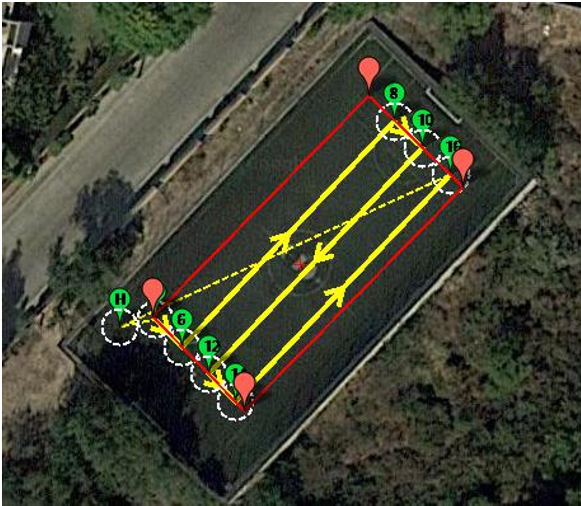
\includegraphics[width=0.7\linewidth]{SummerInterReport/project/Images-Major/flightTraj.png}
    \caption{Flight Trajectory generated by the Mission Planner flight plan tool; Source: \cite{one}}
    \label{fig:compEy}
\end{figure}
Once the drone trajectory is generated by the flight plan tool of the mission planner, the generated system starts covering the area. In order to obtain aerial imagery, the first step is to establish a trajectory that the UAV will follow according to the area of interest. For the trajectory we have used Mission Planner. Mission Planner is a ground station interface compatible with the ArduPilot platform that can be connected to any flight controller based on APM2.8 autopilot. Trajectories can be performed using manual flight modes like STABILIZE, LOITER, and ALT-HOLD. They can also be planned manually using way points at specific locations. These points will guide the UAV. Another way to specify flights trajectories is using polygon points which will automatically generate a flight trajectory covering a desired area. These kind of trajectories are performed in AUTO mode. The flight trajectory used in this procedure will be planned according to the use of polygon points around the area of interest. 
\begin{figure}[H]
    \centering
    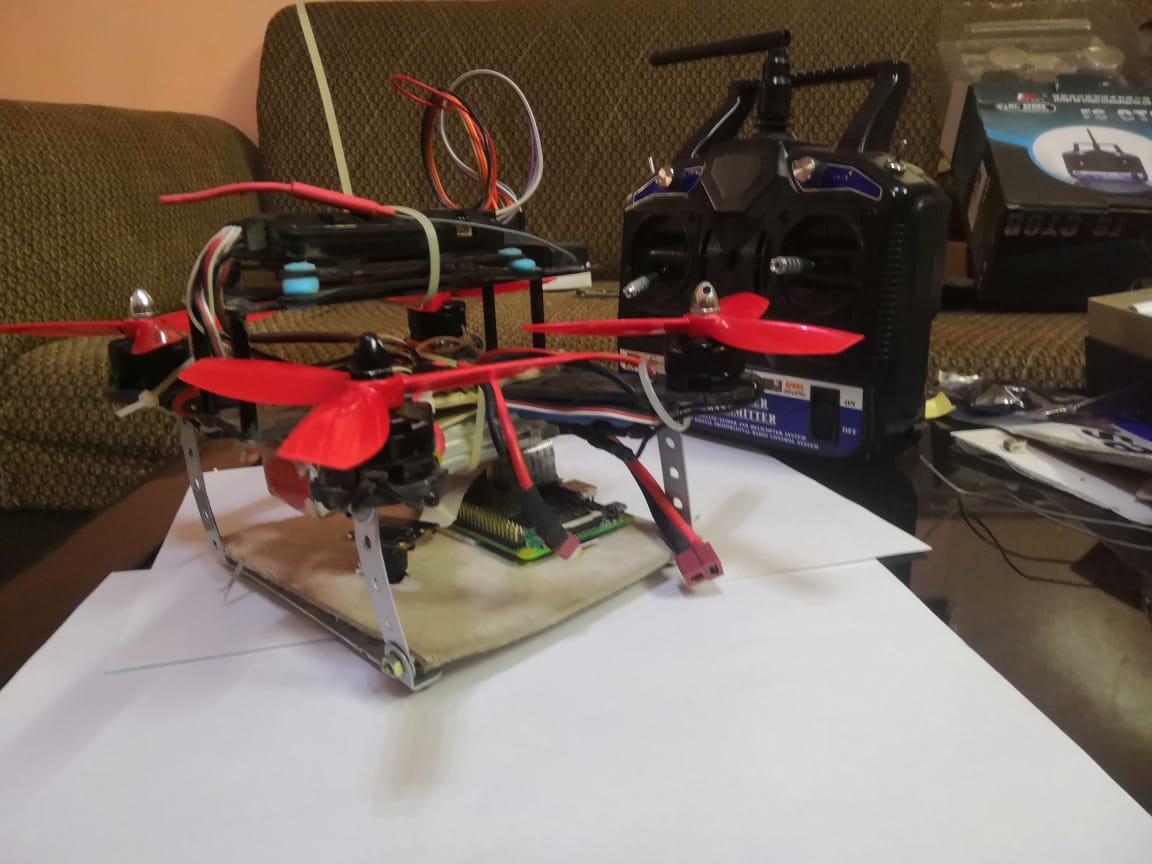
\includegraphics[width=0.7\linewidth]{SummerInterReport/project/Images-Major/complete_drone.jpeg}
    \caption{Complete Drone System generated}
    \label{fig:compEy}
\end{figure}

\section{Data Acquisition and Processing}
The formula to calculate NDVI requires us to know the amount of Near Infrared(NIR) light reflected by the plants and the Red light reflected by the plants. The problem arises when we have to establish such a system on a drone. Hence, it needs to be simple, light and efficient. We worked on three different methods to find out an approximate NDVI keeping in consideration accuracy as well as the cost factor of the overall system.
\subsection{Method 1}
In this method, we acquire the NIR from the Red channel of the Raspberry Pi NoIR camera as it has its infrared filter removed. We use a normal Pi Camera for the identifying the Red light reflected back. But attaching two camera to a Raspberry Pi is not possible without an adapter which costs about Rs. 7000. Rather, attaching two Raspberry Pis is a better and cheaper alternative. Hence each camera has a controlling Raspberry Pi, both triggered to click photos at the same time by the APM2.8
\\
On being triggered, the python script takes a snapshot using the OpenCV package and puts it up on the LAN shared by the two Raspberry Pis using http.server package of Python. Matrix manipulation is done by dividing the difference of the red channel values of both the photos from their sum to calculate NDVI.
\\
NDVI is a ratio from -1 to 1. It is then scaled to range of pixel values(0-255) using the formula (NDVI+1)*255/2. It is then converted to uint8 format from float. After this, the resultant matrix has gradient applied to it using OpenCV and is then further displayed on the web socket

\begin{figure}[H]
    \centering
    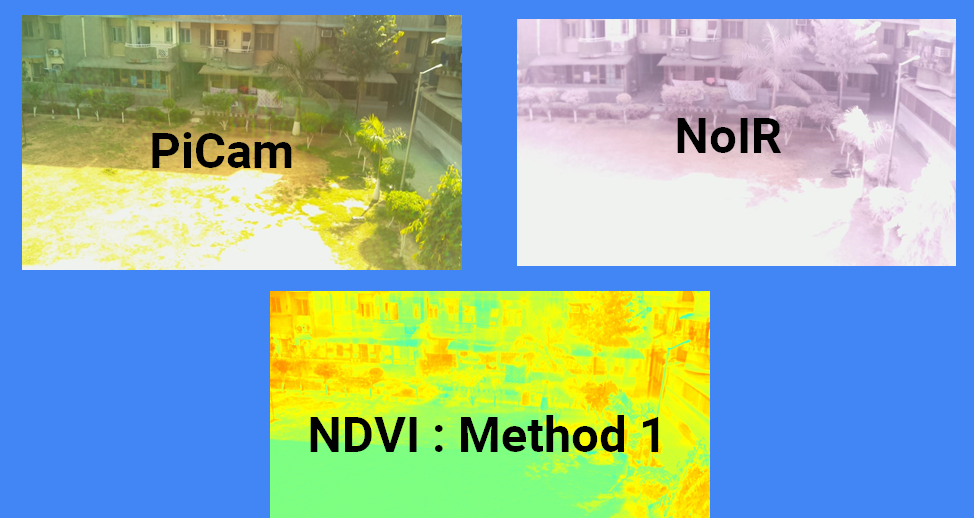
\includegraphics[width=\linewidth]{SummerInterReport/project/Images-Major/ndvi_one.png}
    \caption{Method 1 NDVI calculation}
    \label{fig:compEy}
\end{figure}

\subsubsection{Limitations}
\begin{enumerate}
    \item Connecting two Raspberry Pi leads to synchronization problems in the photos taken due to possible randomly unequal lag supplemented with the dynamics of it being on a drone.
    \item The photos have to be overlapping for the NDVI calculated to be accurate. To achieve this, we need to process the images snapped in accordance to the position of the cameras relative to each other, which may vary from installation to installation, making it a cumbersome task to achieve with high accuracy.
    \item Most importantly, while the formula requires value of NIR reflected, the red channel of the NoIR camera records Red+NIR, leading to a very dampened ratio.
\end{enumerate}
\subsection{Method 2}
In this method, rather than working on individual channels, we work on the intensity of the photos recorded by the two camera. It has the same setup as method 1, but the processing is different. The difference here is that the images are converted to gray-scale for processing.
\\
The conversion of images to gray-scale using OpenCV leads to the images having only one channel. The NIR intensity is replaced by the intensity of the NoIR camera's captured gray-scale image while the Red instensity is replaced by the normal Pi camera's captured gray-scale image to calculate NDVI.
\\
The calculated ratio is then, same as method 1, is mapped to obtain an infographic depicting an approximate value of NDVI

\begin{figure}[H]
    \centering
    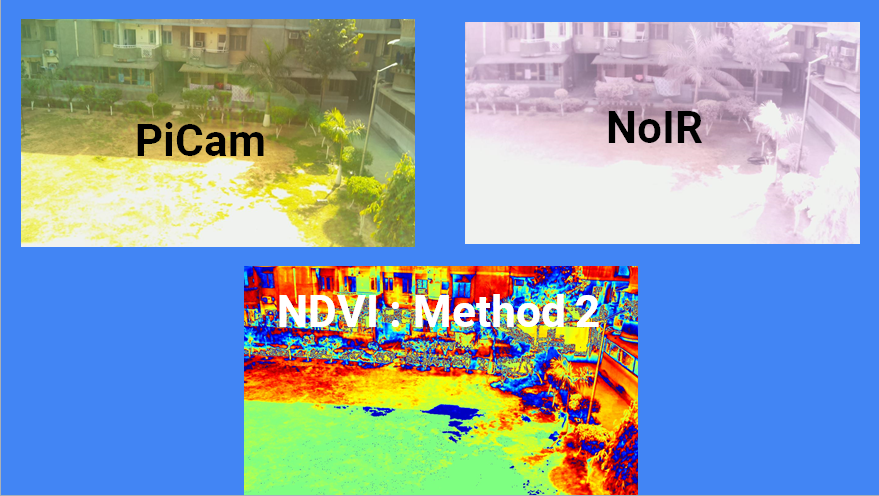
\includegraphics[width=\linewidth]{SummerInterReport/project/Images-Major/ndvi_two.png}
    \caption{Method 2 NDVI calculation}
    \label{fig:compEy}
\end{figure}

\subsubsection{Limitations}
\begin{enumerate}
    \item Same as Method 1
    \item Same as Method 1
    \item It is dependent on light intensity of the images, it is very sensitive to shadows and light intensity changes leading to disparity in calculated NDVI. 
\end{enumerate}
\subsection{Method 3}
NDVI works with Infrared and Red because while Infrared is mostly reflected back by healthy plants, the red light is mostly absorbed by them. But it is not only red light that is absorbed. The leaves(having chlorophyll) also absorb the Blue light, leading to the leaves appearing green to us. Hence, blue light reflected can also be used to calculate NDVI instead of red light.
\\
A blue film filter has the capability to prevent any red light from passing. This in conjunction with the Pi NoIR camera helps us receive intensity of pure NIR(theoretically) in the Red channel of the captured image while we get intensity of Blue light reflected from the blue channel of the image. This type of image is called Infrablue.

\begin{figure}[H]
    \centering
    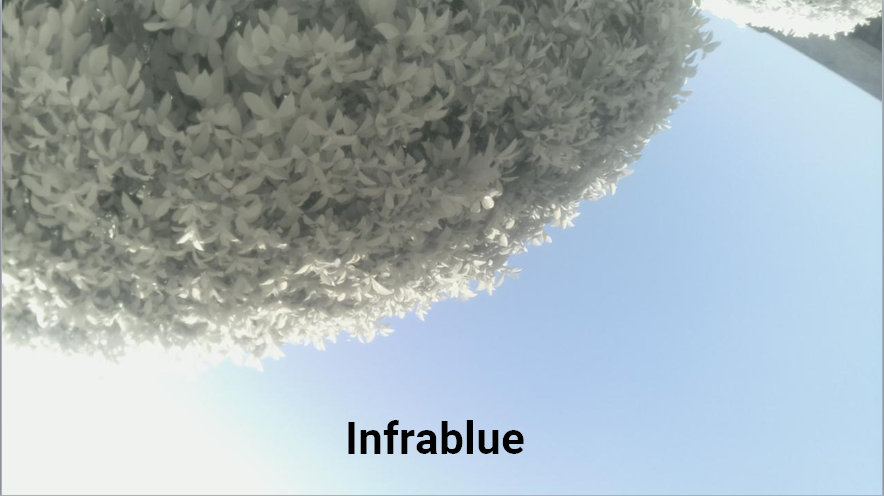
\includegraphics[width=0.7\linewidth]{SummerInterReport/project/Images-Major/infrablue.png}
    \caption{Infrablue Obtained in Method 3 of NDVI calculation}
    \label{fig:compEy}
\end{figure}
\begin{figure}[H]
    \centering
    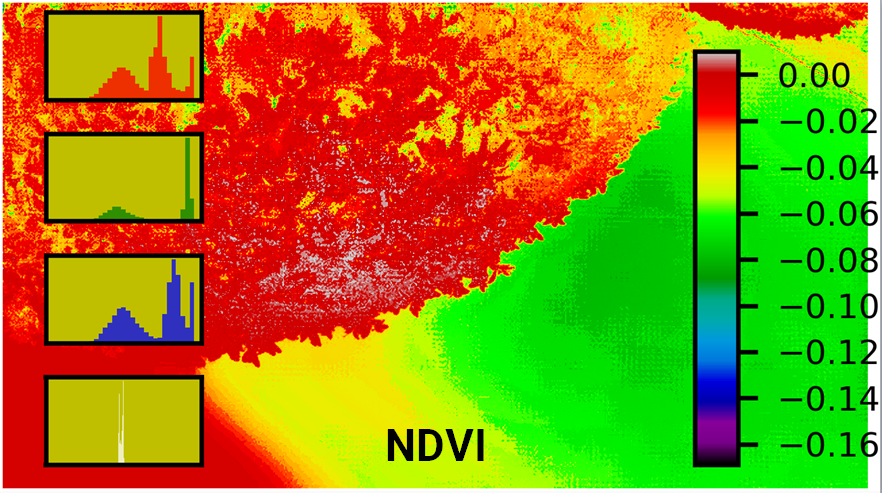
\includegraphics[width=\linewidth]{SummerInterReport/project/Images-Major/ndvi_three.png}
    \caption{Method 3 of NDVI calculation}
    \label{fig:compEy}
\end{figure}

In this method, we require only one Raspberry Pi connected to a Pi NoIR camera with an additional red light filter. The image is captured when triggered by the APM2.8 using OpenCV. Then the NDVI ratio is calculated by using the intensity of blue instead of red and taking intensity of NIR from the red channel of the image. The ratio is then extrapolated to pixel values and a gradient is applied for a pictorial representation in accordance to the minimum and maximum value of the ratio calculated. Further, histograms can be plotted using Matplotlib package for analysing the data.
\\
Method 3 solved all the limitations of the previous methods and proved to be the most optimum method to determine crop health using NDVI.
 % adds the introduction page

%%\section{Implementation}
%\subsection{Drizy - Vision}
% \paragraph{}As mentioned previously, Drizy Vision has been deployed using Raspberry Pi 3 Model B and Raspberry Pi Camera Module V2. This not only makes a cost effective solution but also speeds up the acquisition of frames from the camera since the camera module connects directly to the GPU through the CSI port thereby saving CPU processing for computer vision algorithms.  Drizy Vision has been prototyped for pedestrian-to-vehicle collision avoidance using HOG+SVM \cite{dalal2005histograms} for pedestrian detection that has been implemented using OpenCV and Python2.
% \paragraph{}The HOG (\textbf{H}istogram of \textbf{O}riented \textbf{G}radients)  person detector uses a sliding detection window, 64 pixels wide by 128 pixels tall, which is moved around the image at a predefined step-size. At each position of the detector window, a HOG descriptor is computed. This descriptor is then shown to the trained SVM (\textbf{S}upport \textbf{V}ector \textbf{M}achine), which classifies it as either a pedestrian or not a pedestrian. Before proceeding to further details of implementation, we briefly describe the algorithm for calculation of HOG descriptor. \newline{}\newline{}
% \textbf{CALCULATION OF HOG DESCRIPTOR}\newline{}\newline{} 
% To compute the HOG descriptor, an 8x8 pixel cells are operated on within the detection window. Within a cell, the gradient vector at each pixel is computed.
% \begin{figure}[hbtp]
%   \centering
% %   \vspace{-0.2in}
%     \includegraphics[scale= 0.4]{project/images/image1.png}
%   \caption{\textbf{An 8x8 cell in a 64x128 detection window}}
% \end{figure}
% \newline{}The 64 gradient vectors, in 8x8 pixel cell, is taken and put into a 9-bin histogram. The Histogram ranges from 0 to 180 degrees, so there are 20 degrees per bin. For each gradient vector, it's contribution to the histogram is given by the magnitude of the vector.
% \begin{figure}[hbtp]
%   \centering
%     \includegraphics[scale= 0.5]{project/images/image2.png}
%   \caption{\textbf{9-bin histogram of gradient vectors for an 8x8 cell}}
% \end{figure}
% \newline{}In the next step, the histograms are normalised. However, rather than normalising each histogram individually, the cells are first grouped into blocks of 2x2 and normalised based on all histograms in the block. This block normalisation is performed by concatenating the histograms of the four cells within the block into a vector with 36 components (4 histograms x 9 bins per histogram) and dividing this vector by its magnitude to normalise it. The effect of the block overlap is that each cell appears multiple times in the final descriptor, but is normalised by a different set of neighbouring cells.
% \begin{figure}[hbtp]
%   \centering
%     \includegraphics[scale= 0.7]{project/images/image3.png}
%   \caption{\textbf{Block Normalisation}}
% \end{figure}
% \newline{}The 64 x 128 pixel detection window is divided into 7 blocks across and 15 blocks vertically, for a total of 105 blocks. Each block contains 4 cells with a 9-bin histogram for each cell, for a total of 36 values per block. This brings the final descriptor size to 7 blocks across x 15 blocks vertically x 4 cells per block x 9-bins per histogram = 3,780 values. These values are fed to a trained SVM classifer for detection of object of interest, here pedestrians.
% \paragraph{}The state of art object detection techniques are based on deep learning algorithms like faster R-CNN\cite{ren2015faster}(\textbf{R}egions with \textbf{C}onvolutional \textbf{N}eural \textbf{N}etworks) and its derivatives like YOLO\cite{redmon2016you}. However, the real challenge involves running them real-time on embedded platforms. Therefore, as an acceptable trade-off of 0.8 and 9 (Figure \ref{fig:eval2}) between precision and frames processed per second, respectively, we chose HOG+SVM based pedestrian detector. It has been found that an FPPI (false positives per image) value of 0.5 is acceptable for such driver assistance systems. Figure \ref{fig:eval2} shows that our HOG+SVM pedestrian detector lies well below this threshold at fairly high recall rates.

% \begin{figure}[hbtp]
%   \centering
%   \includegraphics[width=0.5\linewidth]{project/images/roi.png}
%     \includegraphics[width=0.4\linewidth]{project/images/pedestrian.png}
%   \caption{\textbf{Selecting Region of Interest from the Camera view prevents algorithm from detecting all the pedestrians, hence increasing its speed. (b) Detecting pedestrians in ROI using HOG + Opencv}}
% \end{figure}
% \paragraph{}The sliding window algorithm employed for pedestrian detection using HOG+SVM further requires optimisation for bring the fps count to match real-time. Therefore, we reduce the number of sliding windows by selecting region of interest based on known geometric constraints. We achieve further improvement in fps by increasing the step-size of the detection window from 4 pixels to 8 pixels in both x and y direction with nearly no compromise in accuracy. Thus, the processing time for each frame is reduced by a factor of 7x (from 1.4 fps to 9.8 fps). Next, we use multi-threading to parallelize the capture of recent camera frames and pedestrian detection for multiple frames. With the optimised detection techniques, Drizy - Vision is capable of detecting pedestrians within the range of 20 metres.
% % Prototyped on Raspberry pi 3 for pedestrian to vehicle collision avoidance.
% % OpenCV and Python 
% % Used raspberry pi cam to interface directly using camera bus.
% % HOG detector
% % Why no Deep learning?
% % Mention that the assistance system like this requires high fps, and accuracy can be compensated accordingly.
% % Why HOG
% % How far our system detects pedestrians - mention number of windows scanned and all. 
% % Effect of different parameters on fps and stuff 
% % Novelty talks: Optimisation techniques employed
% % Optimisation for embedded platform : ROI, threading, using camera bus
%\subsection{Drizy - Com}
\paragraph{}Drizy - COM has been prototyped for vehicle-to-vehicle collision avoidance alerts at 2 accident blackspots at IIT Delhi. The driver is required to turn on the Drizy smartphone application and turn on the volume. The app starts gathering GPS values from the satellites and infers its attribute like blackspot number, road number etc. The estimate of a potential collision is made on the cloud using a linear predictive algorithm.
\paragraph{}Each vehicle entering a specific accident blackspot uploads its GPS derived attributes via the app to the cloud. The cloud maintains a hierarchical structure of the vehicles and their attributes, as shown in Figure \ref{fig:database}. These attributes include speed and direction of navigation(away or toward the accident blackspot) besides the vehicle's latitude, longitude and altitude. The speed and direction of navigation are determined by studying the change in GPS coordinates of the vehicle. The cloud server refers the cloud database to predict potential collisions in a blackspot and alerts the vehicles that could be on probable collision trajectory. The alerts are sounded on the smartphone itself.
\paragraph{}Algorithm 1 discusses how the server predicts impending collisions and calculates time for each vehicle to reach the intersection point. If the difference in estimated time of any two vehicles to approach the intersection is less than a threshold set to 5 secs, then the cloud sends an alert to vehicles of interest. The alerts are received on the application itself and preset alert tones are generated.\\

% // insert flowchart here
% 			Capture Electronic Horizon from cloud → Capture GPS values from smartphone app → Pre-processes it for blackspot selection (Edge Computing) → Uploads encrypted values to cloud database → Server generates alerts (if any) → Send alerts to Smartphone Application. 

The algorithm adapts its threshold according to the speed of the vehicle. For example, if the vehicle is travelling too fast, then the threshold is doubled to 10 secs, so that driver has sufficient time to apply brakes. This reduces the frequency of alerts thus avoiding redundant or false alerts.

\begin{algorithm}
    	\caption{Server Code Algorithm}
    	\label{Server-Code}
    	\begin{algorithmic}[1]
    		\Procedure{Server Code Algorithm}{$.$}
        	\State {For each pair of vehicles in Accident Black Spot}
        	\State {Get vehicle's GPS, speed, road number from Cloud}
        	\If {$road1!=road2$}
    			\If {direction of both vehicles is toward intersection}
        			\State{Find the distance of two vehicles from intersection using Haversine formula \cite{robusto1957cosine}.}
        			\State{Predict times t1 and t2 to reach the intersection using linear predictive model}
        			 %\State {Predict time difference to reach the intersection using linear predictive model}
        			\If {$|t1-t2|$ $<$ threshold}
        		        \State{Send collision alert to vehicles.}
        			%\State {Move to the next pair}
        			\EndIf
        		\EndIf
        	\EndIf
        	\EndProcedure
    	\end{algorithmic}
    \end{algorithm}
\paragraph{}We used Google Firebase for real-time cloud database maintenance and AWS EC2 UBUNTU 16.04 free tier instance for cloud computing.

% \subsection{Combining Drizy-Vision and Drizy-Com}
% \paragraph{}Drizy-Vision and Drizy-Com function as individual modules. However, the efficacy of the system lies in combining these modules. Combining these two modules synchronizes the alerts from the two individual modules which are then sounded via the buzzer used in Drizy-Vision.
% \paragraph{}The user interface of DRIZY app is provided with a \textbf{PAIR} button to allow users to combine the two modules. This gives raspberry pi access to wifi-hotspot of the phone. Raspberry pi is then connected to the database from where it can download and sound vehicle-to-vehicle collision alerts. The algorithms for warning generation to avoid pedestrian-to-vehicle collision run in parallel. 
% % Deploying Drizy - Vision or Drizy - Com can reduce fatal accidents to half. For users who use the complete Drizy system can synchronize alerts from both the systems and receive all their alerts in Drizy - Vision itself. The Drizy - Com app comes with a PAIR button which uses the WI-FI hot-spot of the smart-phone to connect with Drizy - Vision.
 % adds the Project Design
%\section{Evaluation}

\subsection{DRIZY - VISION}
\paragraph{}This section addresses the question of how well Drizy can detect pedestrians keeping sufficient reaction time for the driver.
\subsubsection{Accuracy}
\paragraph{}Accuracy of a pedestrian detector is generally determined on a frame-by-frame basis. However, Drizy-VISION, a warning system installed in a car, is not affected if all the pedestrians are detected or correctly localized in the frame, instead it validate if an alert is generated when pedestrians walk in front of the car or not.
% We determine the accuracy of Drizy - Vision when a pedestrian detector is used as a warning system in a car. Instead of determining if each pedestrian is accurately localized on a frame-by-frame basis, we validate if an alert is generated when pedestrians walk in front of the car or not.\\
\paragraph{}Using this method, various parameters were evaluated on a video dataset collected on Indian roads with 5500 positives(pedestrians) and 4500 negatives (non-pedestrian/background). All the algorithms were benchmarked on Raspberry Pi 3. Figure \ref{fig:eval2} shows that state of the art techniques like faster RCNN and YOLO offer high precision rates (Equation \ref{eq1}) of 98 to 99 percent with an fps of 0.8 to 1 fps. HOG+SVM classifier (proposed system) provides a speedup 10x over deep learning at a precision of 80 percent.
\paragraph{}Figure 2 shows that HOG+SVM classifier performs better over HAAR with a gain of 0.4 percent recall (Equation \ref{eq2}) at 0.1 FPPI (false positives per image).
\begin{equation}
    Precision = \frac{True Positives}{True Positives + False Negatives}
    \label{eq1}
\end{equation}\\

\begin{equation}
    Recall = \frac{True Positives}{True Positives + False Negatives}
    \label{eq2}
\end{equation}\\

\begin{figure}
\centering
{
\includegraphics[scale=0.85]{project/images/eval2.pdf}
\caption{\textbf{Left: Recall vs FPPI for pedestrian classifiers at varying thresholds. Right: Precision vs frames processed per second for various detection techniques.}}
\label{fig:eval2}
}
\end{figure}
\subsubsection{Reaction Time}
\paragraph{}An alert system should not only detect pedestrians accurately, but also give sufficient to the driver to apply brakes. Here we calculate average reaction time available to the driver from the time of alert to the time of collision with pedestrian.
\paragraph{}The pedestrian detection module is capable of successful detection upto a range of 18 to 23m at varied lighting conditions.A set of experiment was carried out at IIT Delhi campus roads with 50 test drives in a car. The car was maintained at constant speed of 20, 30, 40 and 50km/hr for 10 test drives each. For every drive the time taken to reach the pedestrian after alert reception by Drizy-VISION was noted down. Figure this this this shows that the system warns the driver 4-5 sec prior to approaching a pedestrian ahead at 10-40 km/hr speed limit.
\begin{figure}[hbtp]
\centering
{
\includegraphics[scale=0.6]{project/images/eval1.pdf}
\caption{\textbf{(a) Available Reaction time before collision with pedestrians and vehicles. It shows maximum and minimum values of time obtained during test-runs. (b) Comparative analysis of a system that gives alerts to every vehicle in the accident prone area with DRIZY that predicts collisions before giving alerts. The values were obtained using simulation and spawning of vehicles with random attributes in an accident blackspot.}}
\label{fig:eval1}
}
\end{figure}
\subsection{Drizy - COM}
\paragraph{}This section evaluates Drizy-COM on the basis of the following parameters:\\
(i) available time for driver to apply brake before collision.\\
(ii) frequency of alerts generated by DRIZY. We compare DRIZY with an "Always On" system that gives alerts to every vehicle in the accident blackspot.\\
(iii) accuracy of localization of vehicles. 

\subsubsection{Reaction Time}
\paragraph{}We simulate the same experiment as in Drizy-VISION to analyze reaction time for Drizy-COM at road intersections. We take 50 test drives with 2 vehicles approaching a road intersection from two different roads at varying speed. We analyze the available reaction time for the driver after the collision alert and collision prediction behaviour of the DRIZY app.
Figure \ref{fig:eval1} (a) shows that for speeds limits between 20-25 kmph the system generates alerts with available reaction time >20s and for speed limits reaching 40-45 kmph, it is found to be close to 8s.

\begin{figure}[hbtp]
\centering
{
\includegraphics[width=\linewidth, height=6cm]{project/images/gpserror.png}
\caption{\textbf{Box plot showing deviation in GPS vaues for different mobile phones}
\label{fig:gps}
}}
\end{figure}
\subsubsection{Comparison with "Always On System"}
\paragraph{}In order to study the frequency of collision alerts in different traffic densities, we simulate an experiment. We generate synthetic data with uniform distribution for \lq{N}\rq vehicles which includes vehicle distance from intersection ranging between 0-400m, road number from 0-4, vehicle speed in range 1-36kmph and direction of motion of vehicle. This data is then accessed by the server to predict collisions. Figure \ref{fig:eval1} (b) shows the comparison of DRIZY with an Always On system at low, medium and high density traffic levels. The proposed system reduces the redundant warnings by 80\%, 50\% and 10\% in low, medium and high traffic density, respectively.

\subsubsection{Network Attributes}
\paragraph{}Since the assistance feature is dependent on the network speed, we show the accuracy of GPS data and latencies associated with upload, download and server processing over 4G and WiFi networks. Figure \ref{fig:gps} shows a box plot of GPS errors experimented on different mobile phones. The threshold line shows the maximum tolerable limit in deviation that does not interfere in assistance system. It can be observed that mobile phones launched after 2014 are within the tolerable limit.
\paragraph{}Table 1 shows the latencies of both 4G and WiFi netwoks for different processes. It can be observed that the throughput of the system is not dependent on the type of network or bandwidth of network, it just requires a network connectivity. This behaviour of Drizy-COM is due to the small packet size of the vehicle data that is being uploaded.

\begin{table}[h]
\center
\label{tab1}
 \begin{tabular}{| c | c | c |} 
 \hline
 \multirow{} & \multicolumn{2}{c|}{Time (milliseconds)}   \\\cline{2-3} 
 \textbf{Process} & \textbf{4G} & \textbf{Wifi}\\  
 \hline
 Upload & 258 & 229\\ 
 \hline
 Download & 746 & 678
 \\
 \hline 
 Server processing & 30 & 30
 \\
 \hline
 \end{tabular}
 \caption{Average latency of Drizy-COM for different types of networks.}
\end{table}

\newpage
%\chapter{Creating A Pedestrian Detection Video Dataset On Indian Roads}
\section{Introduction}
\paragraph{} In order to improve the pedestrian detection accuracies as obtained in the Drizy-VISION prototype, we realise that porting the system to use deep learning algorithms is a necessity since these algorithms stand at the forefront when it comes to object detection. With deep learning algorithms becoming a mainstay for vision problems, the need of advanced datasets is a necessity since it is a known fact that deep learning models are data hungry. This means that training these models for pedestrian detection requires a huge pedestrian detection dataset which includes hours annotated video footage of the road scene. All the conventionally available datasets for pedestrian detection (eg. Caltech), however, are recorded in western countries where traffic and pedestrian behaviour is much less chaotic in comparison to countries like India. Hence, we present a pedestrian detection dataset prepared on the roads of New Delhi, India. 
\paragraph{}Further, since creating such a large scale dataset requires hours of manual labour to annotate thousands of frames, we also propose a video annotation tool to minimize the effort required in creating annotations for multi-class, multi-object tracking in chaotic, object dense, occlusion heavy videos. Although the pedestrian dataset does not make use of the full capabilities of this powerful tool, the features that allow creation of a multi-class object tracking dataset are necessary from the perspective of the future extension of our work and are also discussed in detail in the following section. 

\section{Dataset Collection}
As we discussed above that a deep learning algorithm works as good as the data it is fed to train upon. Hence, we propose to use an Indian dataset for training a deep learning model for pedestrian detection to improve the accuracies associated with Drizy-VISION module. The main need of dedicated Indian dataset arises due to these reasons:
\begin{itemize}
     \item High possibility of partial or full occlusion due to heavy traffic
     \item Random movement of Pedestrians across the roads
     \item No separate lanes of pedestrians i.e. cyclists, pedestrians, motorcyclists, cars, heavy vehicles, all run on same roads.
     \item Majority of roads are one-way street and thus pedestrians comes from both the sides.
\end{itemize}
\subsection{Hardware Used}
\paragraph{} The dataset was collected by mounting a WheelWitness HD Pro Dash Cam which has the following features: \\
\begin{itemize}
\item Maximum Video Resolution: Super HD 1296P 2304 X 1296 30 FPS
\item WDR (Wide Dynamic Range) for best night vision
\item 170 Degress, Extra Wide Angle Lens
\end{itemize}
\begin{figure}
\centering
\includegraphics[width=4in, height=2.5in]{SummerInterReport/project/images/dashCam.png}
\caption{\textbf{WheelWitness mounted Dash Cam}}
\end{figure}

It has a Ambarella A7 Processor which allows us to record data on the SD card mounted with recording details and real-time camera feed displayed on the 3.0'' TFT Display. The recording starts as soon as the camera is plugged in to the 12V standard Cigar/Charger point in any car and allows the user to change any setting using the provided push buttons on it.
\subsection{Setup}
\paragraph{}We collected approximately 10 hours of video at 25 fps and resolution 1280 x 720 taken from WheelWitness HD PRO Dash Cam using Ford ECO Sports Car, driving through regular traffic in urban and semi urban streets and roads of New Delhi in dierent lightning conditions over daily commune. The camera was setup on the rear-view mirror of the car giving a central perspective of the road from the vehicle.  

\subsection{Recording Procedure}
\paragraph{} The car was driven normally throughout the recordings. Different drivers were appointed to prevent any driving style bias that might be added otherwise. The video was captured across Paschim Vihar, Rajouri Garden, Punjabi Bagh, Rohini, Noida, driving through DND flyway, Gurugram, Dwarka, Rohtak and some local areas of South Delhi. The video Resolution was of 1280 x 720 pixels which was cropped to 1280 x 300p to remove the sky and lower part of the car (dash-board), to avoid unnecessary computation. The unstabilized instances which occured due to unstable roads were discarded.

\subsection{Annotation Procedure}
\paragraph{} The dataset was annotated using the tool LabelVDOS discussed later in the document. Inspite of the extended abilities of the Video Annotation tool, we have used only single class labelling of pedestrians for detection purposes, including the occlusion label. This setting compares to that of Caltech Dataset and KITTI Benchmark Suite, which some of the most comprehensive dataset for pedestran detection.

\paragraph{} A total of 12539 frames (approx 80 minutes) of data annotation has been completed. In these frames approximately 27000 labelled Bounding Boxes(BBs) of pedestrians were done. Each bounding box(BB) has given two types of labels, pedestrian(23786 BBs) or pedestriano(3182 BBs) denoting unoccluded pedestrians or occluded pedestrians respectively. Since our dataset is still evolving and we are benchmarking it, Indian dataset is not publicly available till date.

\paragraph{} We split Indian dataset into 3 parts, one training and two testing dataset in the ratio of approximately 70\%, 13\% and 17\%. Two testing dataset are created to comment on effect of illumination on results as Test2 dataset have better illumination than Test1. 
\\
\\Table 3.1 Summarizes the whole dataset
\\Table 3.2 Specifies the comparison between Caltech dataset, KITTI Benchmark Suite Dataset and Indian (collected dataset).
\\

\begin{center}
\textbf{Table 3.1 - Dataset Specification}
\begin{table}[!h]
\center
 \begin{tabular}{|c|c|c|c|c|} 
 \hline
 No. & Training & Test1 & Test2 & Total\\ [0.5ex] 
 \hline
 Frames & 8781 & 1551 & 2027 & 12359\\ [0.5ex] 
 \hline
 Non empty Frames & 8164 & 1401 & 1927 & 11492\\ [0.5ex] 
 \hline
 BBs of Pedestrians & 19343 & 3449 & 4176 & 26968\\ [0.5ex] 
 \hline
 Unoccluded & 17065 & 2964 & 3757 & 23786\\ [0.5ex] 
 \hline
 Unoccluded pedestrian per frame & 2.09 & 2.12 & 1.95 & 2.07\\ [0.5ex] 
 \hline
 Unoccluded pedestrian per second & 52.26 & 52.89 & 48.74 & 51.74\\ [0.5ex] 
 \hline
 \end{tabular}
\end{table}
    
\end{center}
\begin{center}
\textbf{Table 3.2 - Dataset Comparison}
\begin{table}[!h]
\center
 \begin{tabular}{|c|c|c|c|} 
 \hline
 No. & Caltech & KITTI & Our \\ [0.5ex] 
 \hline
 Frames & 61439 & 7481 & 12539 \\ [0.5ex] 
 \hline
 Non empty Frames & 61439 & 1779 & 11492 \\ [0.5ex] 
 \hline
 BBs of Pedestrians & 153234 & 4487 & 26968 \\ [0.5ex] 
 \hline
 Unoccluded & 93613 & 4487 & 23786 \\ [0.5ex] 
 \hline
 Unoccluded pedestrian per frame & 1.52 & Not video & 2.07 \\ [0.5ex] 
 \hline
 Unoccluded pedestrian per second & 38.0 & Not video & 51.74 \\ [0.5ex] 
 \hline
 \end{tabular}
\end{table}
    
\end{center}

%\section{labelVDOS : Video Annotation Toolbox}

\paragraph{}
When we look at the existing open source video annotation tools such as ViTBaT \cite{biresaw2016vitbat}, VATIC \cite{vondrick2013efficiently}, ViPER \cite{doermann2000tools} and iVAT\cite{bianco2015interactive}, we find that none of them is suitable due to the complexity and effort in usage, and the high chances of error. It is with this motivation that we create our own tool to label Very Dense Object Sequences (aptly named labelVDOS) with the following novel capabilities:
\begin{itemize}
    % \item The ability to efficiently leverage powerful pre-trained deep learning based object detectors \cite{ren2015faster, liu2016ssd, lin2017focal} to provide bounding box proposals while annotating
    \item The ability to leverage interpolation techniques to only have to correct the bounding box for an object once every few frames, rather than draw one for every frame
    \item The ability to simultaneously keep track of multiple objects without mixing IDs even in dense scenarios
    \item The ability to annotate frame-level phenomenon, making it useful even for tasks such as activity recognition
    \item The ability to work on any platform using just Python
\end{itemize}

The proposed tool, labelVDOS, extends the image annotation tool labelImg\cite{LabelImg} to the particular use-case of creating annotations for object detection as well as tracking in videos. Using an interpolation algorithm, is preferred over an object tracker due to the immense likelihood of ID switches in object dense scenarios which can increase the chances of annotation error. The overall user interface is presented in Figure \ref{labelVDOSLayout} and we now discuss the challenge each component of the tool attempts to solve and its implementation.

\begin{figure}
\centering
{
\includegraphics[width=\linewidth]{SummerInterReport/project/images/labelVDOS_interface.png}
\vspace{-1cm}
\caption{\textbf{The User Interface of Our Proposed Tool}}
\label{labelVDOSLayout}
}
\end{figure}

\subsection{Object Propagation}
In order to ensure that the right-IDs are assigned to the right objects across all frames, we design a Propagation Engine. This Engine ensures that the annotator is able to simultaneously keep track of multiple objects of a wide variety of classes without mixing IDs, even in scenarios that have a high object density. This is accomplished is by ensuring that the bounding boxes that are created on a frame, either by drawing or by accepting proposals, show up on all further frames until the user designates that the object has exited the video.
\paragraph{}The likely location of the bounding box in all future frames is computed by the Propagation Engine using a constant velocity motion model. This allows for users to merely have to correct the positions of bounding boxes in future frames rather than to have to redraw and re-assign their IDs on each frame. 

\subsection{Object Interpolation}
The next challenge that increases the effort of annotators is marking the correct location for all objects in each frame. In order to work around this issue, we design an Interpolation Engine that takes in the bounding boxes of an object in two frames and interpolates all intermediate bounding boxes. We currently use linear interpolation for its simplicity. 
\paragraph{}Suppose that $bbox_{A}$ defines the bounding box in frame A, $bbox_{B}$ in frame B ($A<B$) and let a bounding box be represented as:

\begin{equation}
bbox = [x_{min}, y_{min}, x_{max}, y_{max}]
\end{equation}

Then, for a frame t ($A<t<B$), we can interpolate the bounding boxes using the following equation:

\begin{equation}
bbox_t = \frac{t}{B - A - 1} * (bbox_B - bbox_A) + bbox_A
\end{equation}

In this way, we enable annotators to have to only correct the bounding boxes generated by the Propagation Engine once every few frames, rather than to have to do so on each and every frame.

% \begin{figure*}
% \begin{center}
% \includegraphics[width=0.8\linewidth]{labelVDOSLabelIdSelection.png}
% \end{center}
%   \caption{Annotating a Bounding Box: Selecting from a List of Options. In order to prevent annotators from making errors that arise when typing in labels manually each time, we have them select from a hierarchical list of class labels. This is shown in Figure (A-C). Further, this hierarchy is defined by the Dataset Creators in a simple JSON file which is shipped to all annotators along with the tool. Figure (D) shows this Dataset Creator defined JSON file listing the classes}
% \label{labelVDOSLabelIdSelection}
% \end{figure*}

% \subsection{Object Detector}
% We use the fast and powerful Single Shot MultiBox Detector \cite{liu2016ssd} due to its high speed and reasonable accuracy, allowing it to be run even on CPUs in a reasonable amount of time. Our model is pre-trained on PASCAL VOC, with the option to filter proposals for a relevant set of classes.

% The object detector is used to provide proposals in each frame that do not significantly overlap with ground truth bounding boxes and those from the Propagation and Interpolation Engines. In quantitative terms, we define a metric $IoU_{Proposal}$ for a detection given by:

% \begin{align*}
% IoU_{Proposal} = max(IoU(Proposal, Shape 1), ...,IoU(Proposal, Shape K))
% \end{align*}

% where IoU refers to the ratio of the areas of intersection of two bounding boxes to the area of the union of the two. Only if this metric lies below a tunable threshold $IoU_{ProposalMetric}$, do we display that proposal as a candidate for a new object. 

% Further for those detections for which the metric $IoU_{Proposal}$ lies above a tunable threshold $IoU_{CorrectionMetric}$, we can infer that they refer to the same object as that proposed by the Interpolation or Propagation Engines. Hence, we need to be able to infer which of the two - the detector proposal or the Engine proposal - is more accurate.

% The reason that the detection proposal is not always the more accurate one is that in scenarios with heavy occlusion, the detector merely picks the visible region of the object, while the Engine Proposal which is built from user verified ground truths has a more accurate estimate of the shape of an object. In this way, the Engines complement the Object Detector and this discussion motivates the following metric which helps us decide whether to pick the detection proposal or the engine proposal:

% \begin{equation}
% isOccluded = \frac{Area(Detection)}{Area(Shape)}
% \end{equation}

% In case an object is occluded, then the area of the part that is detected will be much less than the interpolated shape proposed, and thus $isOccluded$ will be small. If, however, the detection has nearly the same area as the shape then it is likely that the detection is more accurate and that will be picked. Hence we have a tunable threshold $isOccludedThreshold$ that will decide whether or not to pick a detection based on the $isOccluded$ metric.

% In this way, the object detector helps provide new proposals as well as complements the Interpolation Engine. Moreover, the use of a deep learning object detector means that the model can be gradually fine-tuned as data is annotated - something that allows for incremental learning as proposed in iVAT.

\subsection{User Interface}

Our tool was designed in Python, focusing primarily on creating a simple interface that would allow users to draw bounding boxes and to have to assign an ID to an object only once. In this way, it would not be difficult for users to keep track of multiple IDs in dense scenarios.
\paragraph{}We keep the UI to be minimalistic and intuitive, in an attempt to minimize the time it takes for the user to create and annotate a bounding box. Moreover, in order to minimize the chances of error involved in marking labels, we allow for the dataset creators to predefine the classes and have the annotators select from a fixed menu of choices. Some of the other key features, apart from the intelligent components like the Propagation and Interpolation Engines include:

\begin{itemize}
  \item The ability to show and hide individual bounding boxes easily, preventing the canvas from becoming especially cluttered
  \item The ability to zoom in and out, which ensures that all relevant objects can be easily selected irrespective of their size
  \item The ability to create multiple bounding boxes without having to click on the draw tool repeatedly
\end{itemize}
\paragraph{}Although our tool has been designed for object tracking in object dense scenarios, it can also be extended to behavior level annotations, as well as handle the frame level annotations required in creating datasets for activity recognition and video captioning.

% Further, the output file is also kept minimalistic, so as to allow the dataset creators to effectively convert the annotations into a format of their choice with minimum effort. Finally, we also include a command to convert the annotations made into a video. This allows both the annotators and the dataset creators to rapidly visualize the entire set annotations for any signs of error.
 
%\addcontentsline{toc}{chapter}{Summary}
%\newpage
\begin{center}
\thispagestyle{empty}
\vspace{2cm}
\LARGE{\textbf{Conclusion and Future Scope}}\\[1.0cm]
\end{center}

\paragraph{}
We started this project with the aim to solve the social problem of road safety in India. It took us no time to realize that it's a long way down the road for driver assistance systems here. To fill these gaps fast, different companies must join hands to create a collaborative system just like it happened a decade ago to create maps. We contributed to this field by implementing Drizy, which is based on the concept of connected cars and computer vision.

\paragraph{}In order to achieve desired accuracies in detecting pedestrians in video input from a dashboard camera as in Drizy-VISION, we took up the challenge of compiling a Pedestrian Detection Video Dataset recorded on Indian roads to train deep learning models. Realising that the existent video annotation toolboxes did not fill in our needs, we also launched our very own customised toolbox - labelVDOS.

\paragraph{}The future prospects of our project include determining and improving the accuracies of existent object detection models like Faster RCNN by fine tuning them on the Indian Pedestrian Detection Dataset. We also wish to extend our work for Pedestrian Trajectory Estimation. 
% \paragraph{}The system finds its utility even in bad weather conditions since prediction of collisions at intersection points is based on vehicle-to-cloud communication. On the other hand, the functionality of Drizy-VISION is aimed specifically to aid distracted drivers. Although Drizy has currently been prototyped for two types of assistance features only, the applicability of the system can be expanded using the same framework.
% \paragraph{}Initial stages in developing Drizy-COM involved experiments on setting up peer-to-peer networks over ZigBee protocols. However, this limited communication between vehicles in the range of 60-70 metres. These networks would also be limited to vehicles on a straight road, whereas at bends, obstacles like buildings would hinder communication. Therefore, communication over cloud was chosen due to its robustness. Latency issues related to data uploading, cloud-computing and data downloading were dealt with by employing the concept of edge-computing.
% \paragraph{}Results validated that a collaborative driver assistance system is feasible in low and medium traffic density. The current system design could be limited merely by computation power of raspberry pi and internet connectivity. It is independent of internet speed due to extremely small packet of data being uploaded and downloaded. Optimizations implemented to speed up computation on embedded systems could make such systems cost-effective. Thus, such systems are easily deploy-able and will be the future of driver assistance systems in developing countries with complex road conditions. They could be a solution to improving road safety and achieving the target of lowering road accidents and fatalities to half by 2020. 
% In future, we plan to design a peer-to-peer network of cars which can help overcome the dependency of the system on internet connection which is still a matter of concern in certain areas in developing countries. In order to increase the utility of the system, we also plan to add a feature that helps vehicles on a road to coordinate and clear out the way for ambulances to pass, thereby creating a "Green Corridor". \\
%Not sure of this above statement
% This can be our future work. But i doubt if we will actually do it. Same. even the green corridor thing . Lets just add then.Okay. Also, i have sent the TODO list on hangouts.Oh okay. I will keep myself involved in presentations and videos for the next week. let me know if you can help me in this. Sure I . have a look at snapchat for element of hapiness. downloading snapchat lol. rehne de, insta kar diya. refreshing insta
% As discussed earlier, Raspberry Pi 3 with limited compute power was not sufficient for heavy processing involved in state-of-art computer vision algorithms based on deep learning. With a trade-off between speed and accuracy we designed Drizy which can alert the driver of impending collision with pedestrians and other vehicles.\\
% The system finds its utility in bad weather conditions when the driver has limited visibility or may not be paying attention to its environment.\\
% The major challenges we faced in the project includes limited network bandwidth and poor visibility of lane markings. However, they were both taken care of using concepts like edge computing and image segmentation.\\
% Drawbacks of Drizy includes its lack of communicating with cars which do not have Drizy installed. This may reduce the overall utility of the system. In future we plan to design a peer-to-peer network in cars which can overcome this drawback and decrease latency.
 

\chapter{Conclusion and Future Scope}
\section{Conclusion}
A complete drone end-to-end service was designed for the use of multispectral imagery. We developed a bilingual android application with easy to use interface for the farmers to call drones and view infographic information of the crop fields, test drones with different flight controllers and a data acquisition and processing system on-board the drone. We figured out the best board to use in the scenario as the cheapest alternative is ArduPilot APM2.8 with GPS enabled. The board was fixed on a custom made 250 mm carbon fibre chassis. The data acquisition system costed around 50\$ making it one of the cheapest multispectral imagery set-up. We tested the drone in open environments and assessed the crop health as well. Providing it as a service increases the feasibility of the proposed solution in the Indian market.
\section{Future Scope}
The future work involves improvisations and optimizations to the existing framework of multispectral imagery with addition of designated Thermal Sensors like AMG833 to calculate the water stress levels and Hyper-spectral cameras like Rikola Hyperspectral cameras along with Machine Learning Clustering algorithms to find out elemental deficiencies and potential crop diseases.
\\
We also tend to incorporate the satellite modules for remote sensing modularity added in the mainframe. Satellite imagery can also help us assess the temporal features of the crops which act as an important delimiter in the yield and overall health assessment of the soil.
%add 'em

% Our work is future proof and cost effective
% User independent
% Cost-effective
% Easily deployable
% The system helps us achieve our target, of 250-million connected vehicles by 2020, using a robust framework.
% How we make a dent and why should someone buy the system  % adds the Scheduling and Planning page
% \bibliographystyle{unsrt} % adds the References page
% \bibliography{referencebib}
\addcontentsline{toc}{chapter}{References}
\begin{thebibliography}{}
\bibitem{one}Andres Montes de OcaLuis, Arreola Alejandro, FloresShow, Gerardo Flores, "Low-cost multispectral imaging system for crop monitoring" in Conference: ICUAS'18 The 2018 International Conference on Unmanned Aircraft Systems at Dallas, TX, USA, May 2018

\bibitem{two}Adao, T., Hruska, J., Padua, L., Bessa, J., Peres, E., Morais, R. Sousa, J.J., " Hyperspectral Imaging: A Review on UAV-Based Sensors, Data Processing and Applications for Agriculture and Forestry." in Remote Sens. 2017, 9, 1110. 

\bibitem{eight_icuas}A. M. Jensen, M. Baumann, and Y. Chen, "Low-cost multispectral aerial imaging using autonomous runway-free small flying wing vehicles," in IGARSS 2008 - 2008 IEEE International Geoscience and Remote Sensing Symposium, vol. 5, July 2008, pp. V - 506-V - 509

\bibitem{two_remotev2}Park, S., Nolan, A., Ryu, D.; Fuentes, S., Hernandez E., Chung, H., O'Connell M., " Estimation of crop water stress in a nectarine orchard using high-resolution imagery from unmanned aerial vehicle (UAV)" In Proceedings of the 21st International Congress on Modelling and Simulation, Gold Coast, Australia, 29 November–4 December 2015; pp. 14131419. 

\bibitem{three_remotev2}Primicerio, J., Gennaro, S.F. D., Fiorillo E., Genesio, L., Lugato, E., Matese, A., Vaccari, F.P., " A flexible unmanned aerial vehicle for precision agriculture" Precis. Agric. 2012, 13, 517–523

\bibitem{fourteen_remotev2}Multispectral vs. Hyperspectral Imagery Explained. Available online: http://gisgeography.com/ multispectral-vs-hyperspectral-imagery-explained/ (accessed on 15 September 2017). 

\bibitem{fifteen_remotev2}Proctor C., He, Y., " Workflow for Building A Hyperspectral Uav: Challenges And Opportunities", ISPRS Int. Arch. Photogramm. Remote Sens. Spat. Inf. Sci. 2015, XL-1/W4, 415–419. 

\end{thebibliography}

\end{document}